\documentclass{beamer}

\usepackage[utf8]{inputenc}
\usepackage{default}

\mode<presentation>
%{ \usetheme{boxes} }


\usetheme{Madrid}

\usepackage{times}
\usepackage{graphicx}
\usepackage{tabulary}
\usepackage{listings}
\usepackage{verbatimbox}
\usepackage{graphicx}
\usepackage{lmodern}
\usepackage{bm}
\usepackage[absolute,overlay]{textpos}
\usepackage{pgfpages}
\usepackage{color}
\usepackage{amsmath}
\usepackage{multicol}
\usepackage{stmaryrd}

\definecolor{mycolorcli}{RGB}{53,154,26}
\definecolor{mycolorcode}{RGB}{0,0,255}
\definecolor{mycolordef}{RGB}{255,0,0}

\newcommand{\mycode}[1]{{\color{mycolorcode}#1}}
\newcommand{\mycli}[1]{{\color{mycolorcli}#1}}
\newcommand{\mydef}[1]{{\color{mycolordef}#1}}

\newcommand{\mycodeb}[1]{{\color{mycolorcode}\textbf{#1}}}
\newcommand{\myclib}[1]{{\color{mycolorcli}\textbf{#1}}}
\newcommand{\mydefb}[1]{{\color{mycolordef}\textbf{#1}}}


\pgfdeclareimage[height=0.65cm]{logo_rcc}{graphs/logo_rcc.png}
\setlength{\TPHorizModule}{1mm}
\setlength{\TPVertModule}{1mm}
\newcommand{\RCCLogo}{
\begin{textblock}{14}(1.5,1.5)
  \pgfuseimage{logo_rcc}
\end{textblock}
}


\title{\huge{GPU programming with CUDA}}
\author{Igor Yakushin \\ \texttt{ivy2@uchicago.edu}}

\definecolor{ChicagoMaroon}{RGB}{128,0,0}

\setbeamercolor{title}{bg=ChicagoMaroon}

\begin{document}

\setbeamertemplate{navigation symbols}{}

\setbeamercolor{fcolor}{fg=white,bg=ChicagoMaroon}
\setbeamertemplate{footline}{
\begin{beamercolorbox}[ht=4ex,leftskip=1.4cm,rightskip=.3cm]{fcolor}
\hrule
\vspace{0.1cm}
   \hfill \insertshortdate \hfill \insertframenumber/\inserttotalframenumber
\end{beamercolorbox}
}

\setbeamercolor{frametitle}{bg=ChicagoMaroon,fg=white}

\begin{frame}
\RCCLogo
\titlepage
\end{frame}


\section{How to get the tutorial and log into midway 2}
\begin{frame}[fragile]
  \frametitle{How to get the tutorial and log into midway 2}
  \begin{itemize}
  \item Point your browser to
    {\small
      {\color{mycolorcli}
\begin{verbatim}
https://git.rcc.uchicago.edu/ivy2/cuda
\end{verbatim}
      }
    }
    \item If you have RCC account and allocation, login to midway 2 as usual: 
{\color{mycolorcli}
\begin{verbatim}
ssh -Y <username>@midway2.rcc.uchicago.edu
\end{verbatim}
}
\begin{itemize}
\item For more details, see:
  {\color{mycolorcli}\verb|https://rcc.uchicago.edu/docs/connecting/index.html|}
\end{itemize}
\item If you do not have RCC allocation, use yubikey: {\color{mycolorcli}\verb|https://git.rcc.uchicago.edu/ivy2/yubikey|}
\item Once on midway 2, clone the tutorial with the labs:
    {\small
      {\color{mycolorcli}
\begin{verbatim}
git clone https://git.rcc.uchicago.edu/ivy2/cuda.git
\end{verbatim}
      }
    }
    \item The labs are in  {\color{mycolorcli}\verb|cuda/labs|}
    \item The presentation is in  {\color{mycolorcli}\verb|cuda/docs/CUDA.pdf|}
%    \item Set up the environment {\color{mycolorcli}\verb|source cuda/labs/env.sh|}
    \end{itemize}
  \end{frame}

%
\section{Content}
\begin{frame}[fragile]
  \frametitle{Content}

\begin{itemize}
\item The tutorial is organized as a spiral: 
  \begin{itemize}
    \item For example, rather than presenting everything about parallel algorithms in one big section, we shall keep revisiting algorithms periodically at each circle of the spiral, introducing more and more complicated
      topics
    \item At each circle of a spiral we shall try to present enough material about GPU architecture, CUDA programming and parallel algorithms to reach the next level in our understanding of GPU programming and to be able to do 
      the next lab
    \item We shall keep moving around the spiral until we run out of topics, audience or time whatever comes earlier.
  \end{itemize}
\end{itemize}
\end{frame}



\begin{frame}[fragile]
  \frametitle{Content}
\begin{itemize}
\item The tutorial covers the following topics, not necessarily in this order:
  \begin{itemize}
    \item GPU architecture:
      \begin{itemize}
      \item Organizing computation into threads, blocks, warps, grid; what is Streaming Multiprocessor (SM), compute capability
      \item Memory organization: host memory, GPU global and local memory, shared memory, registers, texture and surface memory, constant memory, cache
      \end{itemize}
    \item Parallel algorithms: strong and weak scaling, Amdahl and Gustavson laws, map, reduce, scan (inclusive, exclusive), histogram, compact, sort, 
    \item CUDA programming: 
      \begin{itemize}
        \item creating and launching kernels
        \item moving data between host and device, unified memory
        \item using streams to interleave computations and data moving
        \item dynamic parallelism
        \item optimizing CUDA program
        \item debugging and profiling CUDA program with {\color{mycolordef}nvidia nsight tools}
        \item using CUDA accelerated libraries like {\color{mycolorcode}cublas}, {\color{mycolorcode}cusparse}, {\color{mycolorcode}thrust}
        \item compiling CUDA programs with {\color{mycolorcli}nvcc}
      \end{itemize}
  \end{itemize}
\end{itemize}
\end{frame}

\section{Why to use parallel programming?}
\begin{frame}[fragile]
  \frametitle{Why to use parallel programming?}
  \begin{itemize}
  \item Until 2005, CPU frequency kept doubling every year or so and your old sequential program would automatically run faster on the new hardware without you having to do anything.
  \item This is no longer true: we cannot keep increasing CPU frequency since we cannot handle so much heat per unit area.
  \item As a result, during recent decade the progress in computing hardware was in increasing degree of parallelism by using wider vectors, 
    more CPU cores, offloading computations to accelerators such as GPUs, TPUs, FPGAs, using faster memory, 
    increasing bandwidth between memory and CPU or CPU and accelerators, 
    using faster interconnect between nodes in a cluster to be utilized, for example, by MPI or other distributed computing framework.
  \item Your old sequential program will not run any faster on the new hardware unless 
    you redesign it to utilize the available parallelism.
  \item Offloading part of computation to GPU is one way to speed up your program, potentially by $10^n$.
  \end{itemize}
\end{frame}

\begin{frame}
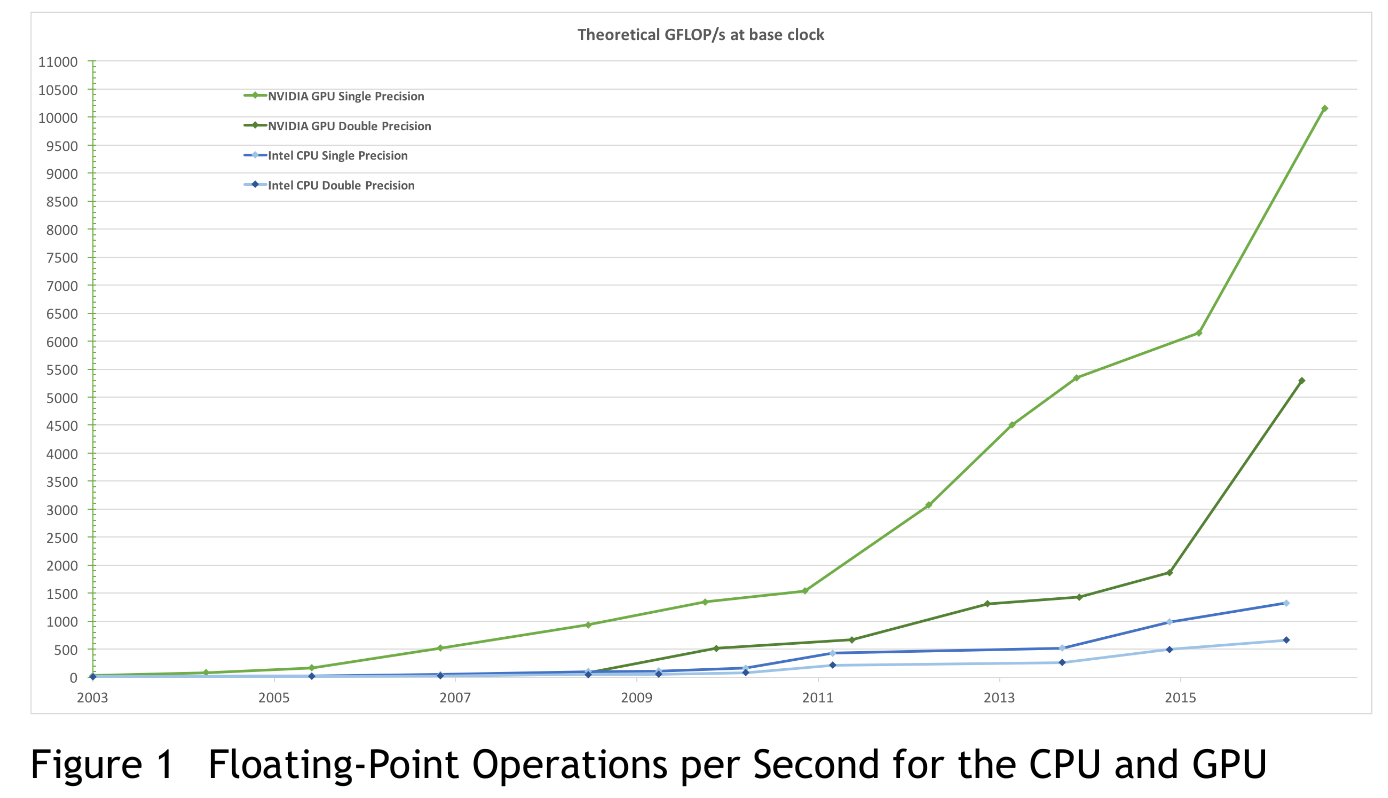
\includegraphics[width=11.5cm]{graphs/fps.png}
\end{frame}


\begin{frame}
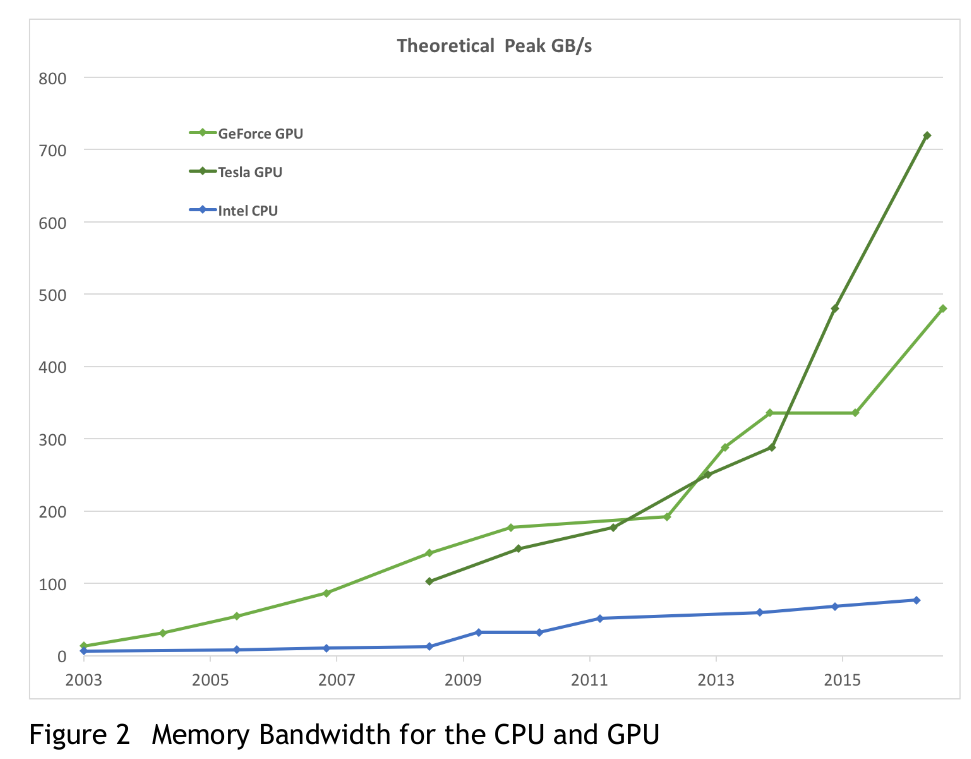
\includegraphics[width=11.5cm]{graphs/bps.png}
\end{frame}

\section{Scaling}
\subsection{strong}
\begin{frame}[fragile]
  \frametitle{Scaling: strong}
\begin{itemize}
\item By how much can one speed up a program using $N$ processors, if the program spends $P$ fraction of its time in the part of the code that can be parallezed?
\item Assuming the best case of {\color{mycolordef}linear scaling}:
\begin{equation*}
speedup = \frac{P + (1 - P)}{\frac{P}{N} + (1 - P)} = \frac{1}{\frac{P}{N} + (1 - P)}
\end{equation*}
\item The above equation is called {\color{mycolordef}Amdahl's law}, it describes {\color{mycolordef}strong scaling} - how faster can one do a fixed amount of work given more processors.
\item Obviously, the bigger is $P$, the more sense it makes to spend efforts parallelizing the corresponding part of the code.
\item For example, assuming the best case $N=\infty$ and linear scaling, if $P=0.99$, $speedup = 100$; however, if $P=0.5$, $speedup=2$. 
\item In reality, linear scaling is too optimistic and is often limited by communication overhead, synchronization, memory bandwidth, etc.
\end{itemize}
\end{frame}

\subsection{weak}
\begin{frame}[fragile]
  \frametitle{Scaling: weak}
\begin{itemize}
\item Often we are interested in a different question: given more processors, how much more work 
  can we do during the fixed amount of time? 
This is called {\color{mycolordef}weak scaling} and is described by {\color{mycolordef}Gustafson's law}.
\begin{equation*}
morework = \frac{P*N + (1 - P)}{P + (1 - P)} = P*N + (1 - P)
\end{equation*}
\item 9 women producing 1 baby in 1 month - strong scaling
\item 9 women producing 9 babies instead of 1 baby in 9 months - weak scaling
\item Again, linear increase of the amount of work with the number of available processors is usually too optimistic: 
  there will likely be bottlenecks in communication bandwidth, synchronization, etc. that would limit strong scaling.
  For example, if there are 4 lanes in the road, only 4 cars can travel in parallel.
\end{itemize}
\end{frame}

\section{GPU hardware}
\subsection{Thread, warp, block, grid, SM}
\begin{frame}[fragile]
  \frametitle{GPU hardware: thread, warp, block, grid, SM}
\begin{itemize}
\item GPU consists of several {\color{mycolordef}Streaming Multiprocessors (SMs)}
\item Each SM can run several thousand GPU {\color{mycolordef}threads} in parallel
\item For example, V100 has 80 SMs, K80 has 13 SMs. Each SM in those can run up to 2048 threads. Therefore up to 163840 threads can run in parallel in V100 and up to 26624 threads in K80.
\item GPU cores have much simpler logic than CPU core: do not do branch prediction, less caching
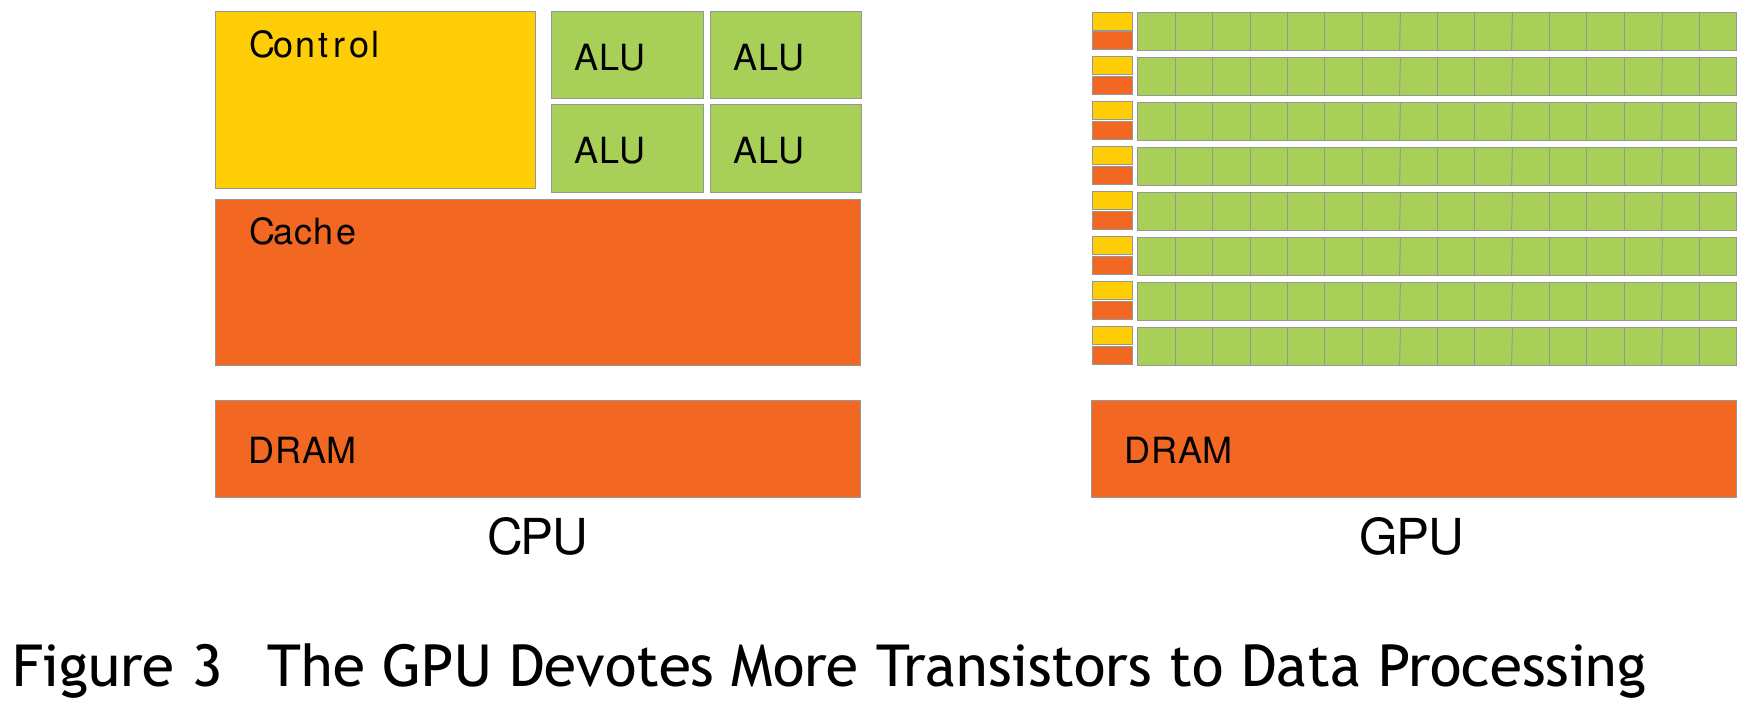
\includegraphics[width=8.5cm]{graphs/gpu_vs_cpu.png}
\end{itemize}
\end{frame}


\begin{frame}[fragile]
\begin{itemize}
\item Each GPU core is a few times slower than CPU core. For example, V100's clock frequency is 1.530 GHz, K80's - 0.824 GHz, while typical CPU clock frequencies today are around 2.5 - 3.0 GHz.
\item The threads in a job are grouped into a {\color{mycolordef}grid of blocks}
\item Each block can have up to 1024 threads
\item Blocks are scheduled to run on SMs in no particular order, in parallel  or sequentially, on the same SM or on different SMs
\item The whole block runs on one SM
\item Inside a block, threads are grouped into {\color{mycolordef}warps}
\item In a warp, there are 32 threads
\item Hardware executes each warp as a single entity
\item It is best if threads in a warp do not diverge but do the same instruction at each step
\item In case of a thread divergence in a warp due to {\color{mycolorcode}\verb|if|} statements or different lengths of loops, the divergent parts are executed sequentially
\item This architecture of GPU is called {\color{mycolordef}SIMT - Single Instruction Multiple Threads}
\end{itemize}
\end{frame}

\begin{frame}[fragile]
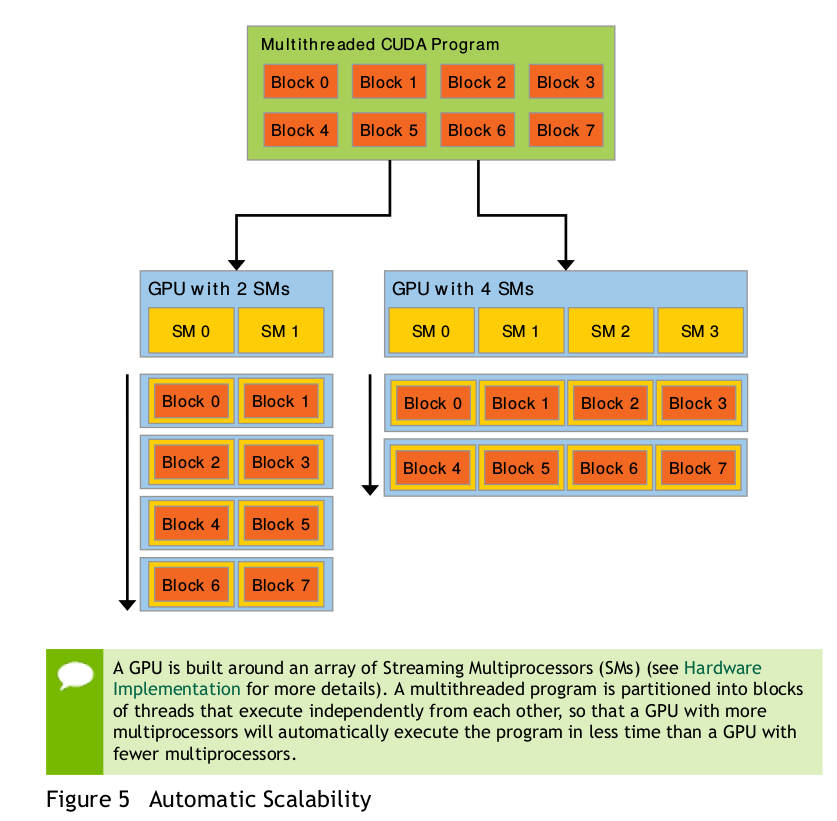
\includegraphics[width=9.0cm]{graphs/blocks_per_sm.png}
\end{frame}

\begin{frame}
\begin{columns}
\begin{column}{0.55\textwidth}
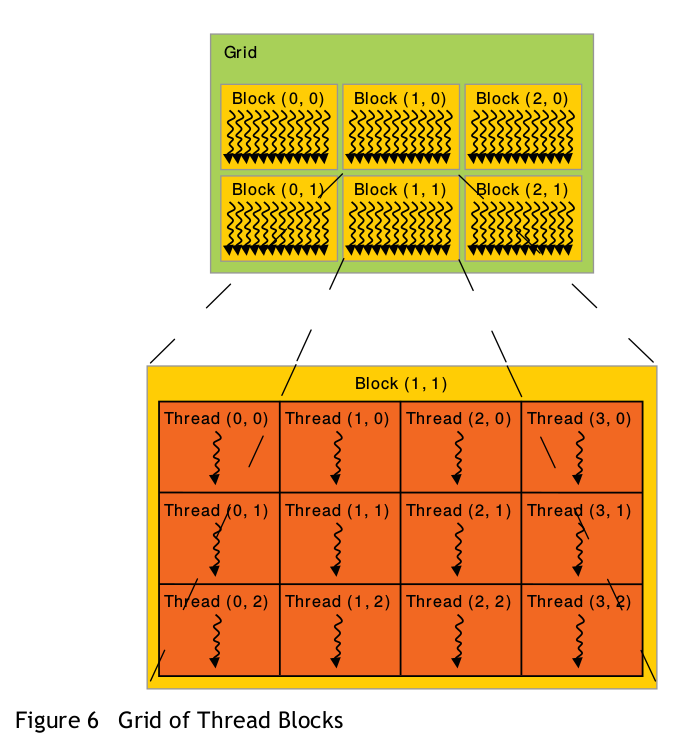
\includegraphics[width=6.5cm]{graphs/grid_of_blocks.png}
\end{column}
\begin{column}{0.45\textwidth}
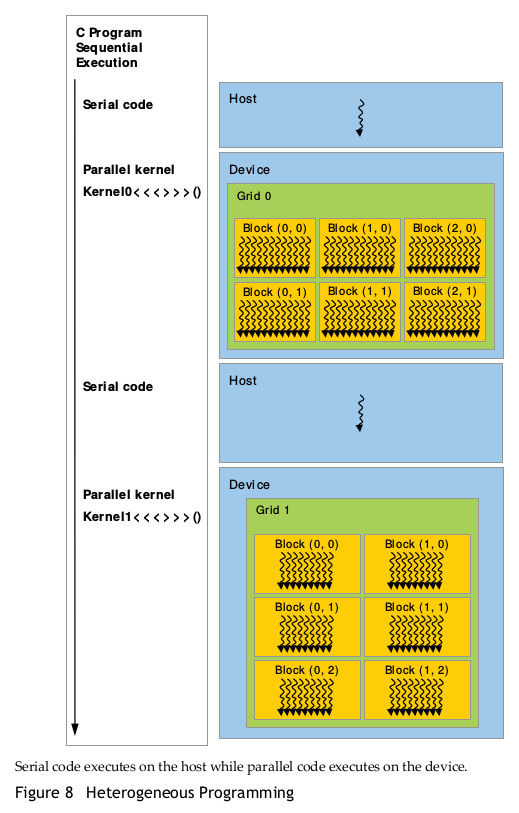
\includegraphics[width=5.5cm]{graphs/heterogeneous.png}
\end{column}
\end{columns}
\end{frame}




\subsection{Memory}
\begin{frame}[fragile]
  \frametitle{GPU hardware: memory}
\begin{itemize}
\item GPU uses its own memory - {\color{mycolordef}global memory}
\item One might have to copy data between CPU host and GPU device.
\item K80 has 12G, V100 - 16G
\item The bandwidth between global memory and GPU for K80 is $480GB/s$, for V100 - $900GB/s$
\item For comparison: the typical bandwidth between CPU and RAM is about $100GB/s$
\item GPU card is typically connected to CPU host with PCI interface with a bandwidth of about $12GB/s$, for PCIe gen3 - $32GB/s$
\item There are faster interconnects  available, for example, {\color{mycolordef}NVlink} - $300GB/s$, but so far they are too expensive and not
  yet widespread and transferring data between CPU and GPU is likely to be the biggest bottleneck for a while
\item Therefore to get better performance, one needs to minimize moving data between the host and device or interleave it with the computations to hide the latency

\end{itemize}
\end{frame}


\begin{frame}[fragile]
  \frametitle{GPU hardware: memory}
\begin{itemize}
\item Given the number of threads, global memory is slow and one needs to minimize its usage as well
\item One way to optimize usage of global memory is {\color{mycolordef}coalescing}: take into account that data is read from global memory in {\color{mycolordef} aligned cache lines} and in ideal close threads should read close data
\item Per block, there is faster {\color{mycolordef}shared memory}, limited to $48k$ for K80 and $96k$ for V100. It can be used to cache global memory values manually.
\item Local variables in a thread are kept in {\color{mycolordef}registers} which are faster than shared memory. 
  However, there is limited amount of registers available and some local variables might spill into {\color{mycolordef}local memory} which physically resides in the same place as global
  memory and therefore is as slow.
\item {\color{mycolordef}Constant memory} is optimized for read operations although physically it is still the same as global memory.
\item {\color{mycolordef}Texture and surface memory} are used mostly for graphics programming and we shall not discuss it here.
\end{itemize}
\end{frame}


\begin{frame}[fragile]
  \frametitle{GPU hardware: memory}
\begin{columns}
\begin{column}{0.5\textwidth}
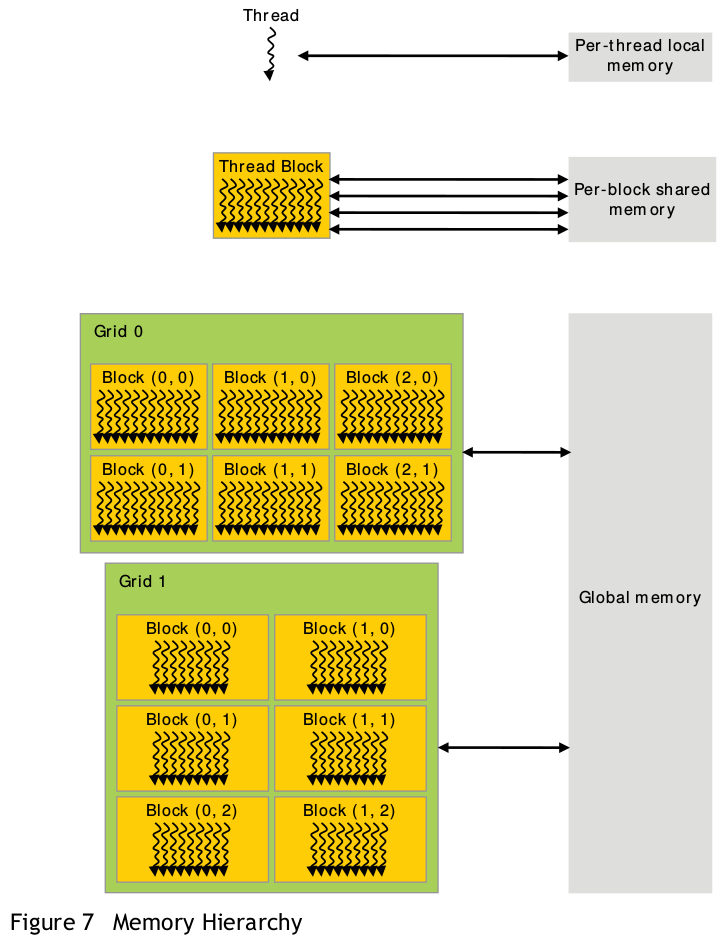
\includegraphics[width=6.0cm]{graphs/memory_hierarchy.png}
\end{column}
\begin{column}{0.5\textwidth}
\begin{itemize}
\item The host can only copy data to/from global, constant, texture, surface memory; not shared memory, registers or local memory
\item For optimal performance, it is important to {\color{mycolordef}align} data in memory since reads and writes start at aligned address
\item Builtin types are aligned automatically but user defined types like structures might have to be aligned manually
\end{itemize}
\end{column}
\end{columns}
\end{frame}

\begin{frame}[fragile]
  \frametitle{GPU hardware: memory}
\begin{columns}
\begin{column}{0.5\textwidth}
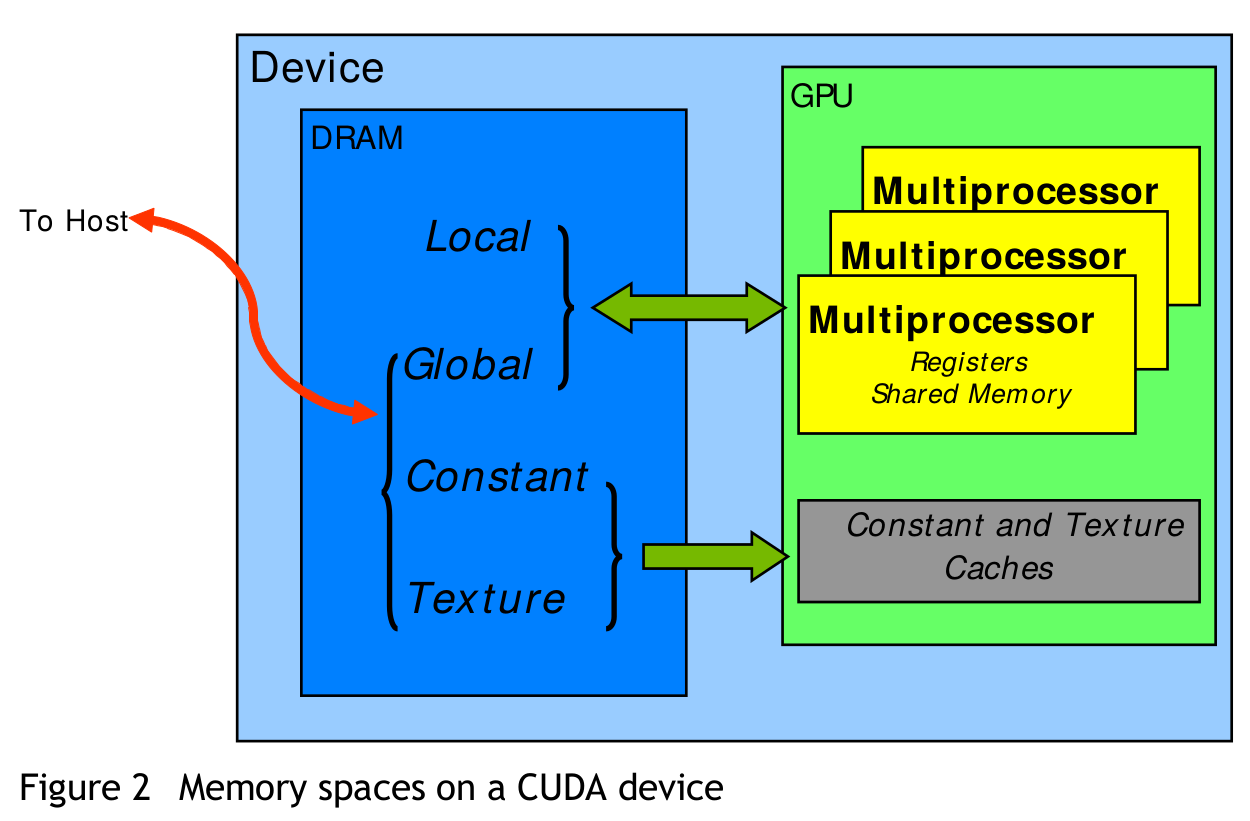
\includegraphics[width=4.0cm]{graphs/memory2.png}
\end{column}

\begin{column}{0.5\textwidth}
\begin{itemize}
\item {\color{mycolordef}Unified Memory}, available for $CC \ge 3.0$,  allows using the same pointer both on the host and device and makes data transfer transparent for the user. 
\end{itemize}
\end{column}

\end{columns}
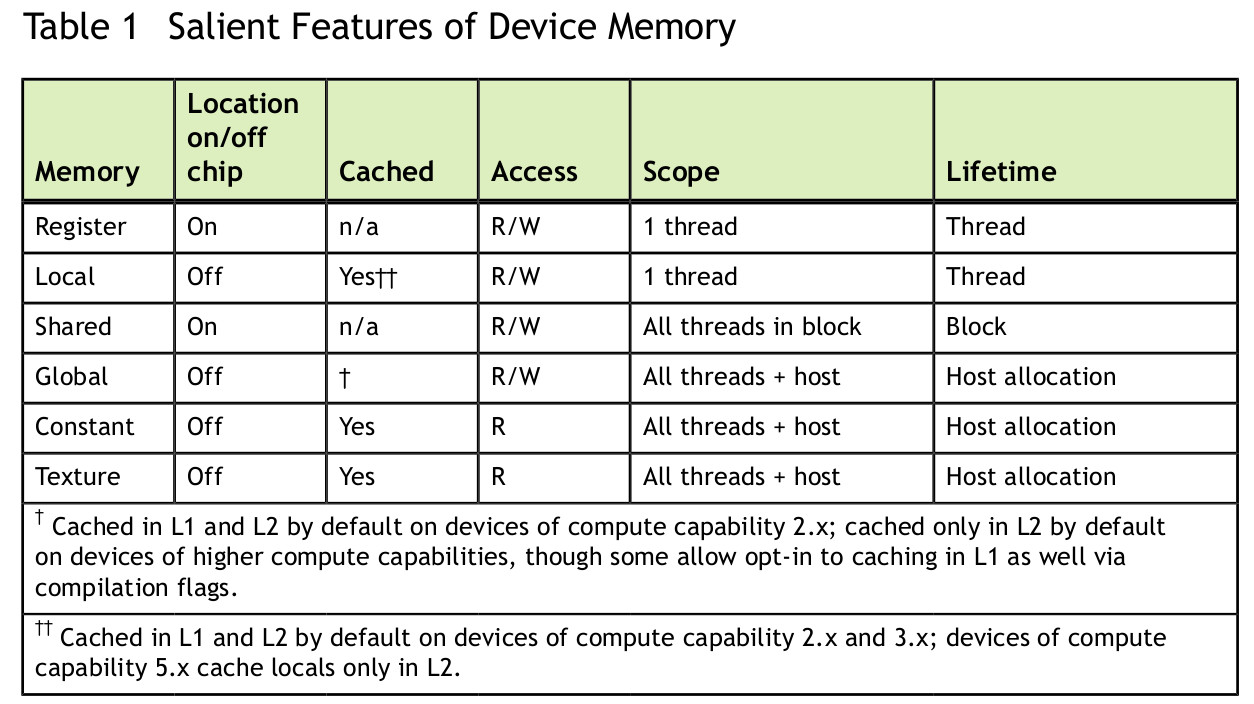
\includegraphics[width=9.0cm]{graphs/memory3.png}
\end{frame}


\begin{frame}[fragile]
  \frametitle{GPU hardware: memory}
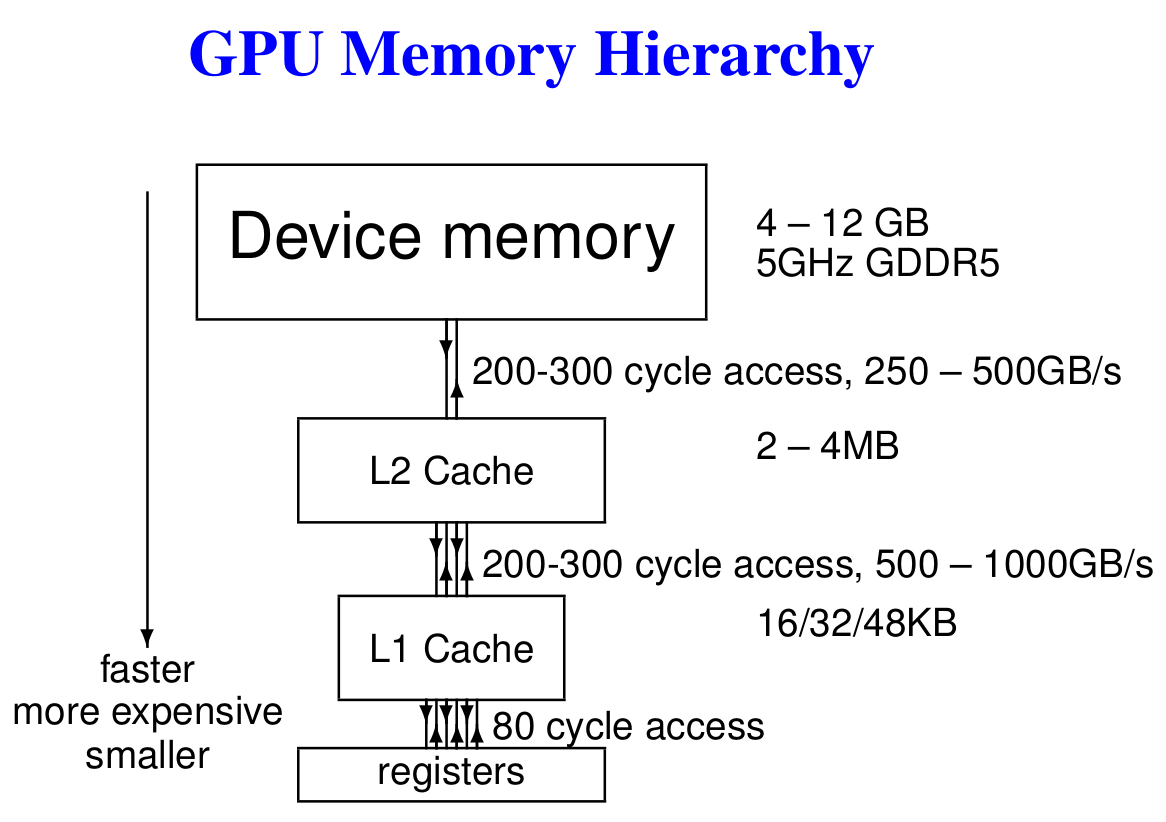
\includegraphics[width=11.0cm]{graphs/memory5.png}
\end{frame}

\begin{frame}[fragile]
  \frametitle{GPU hardware: memory}
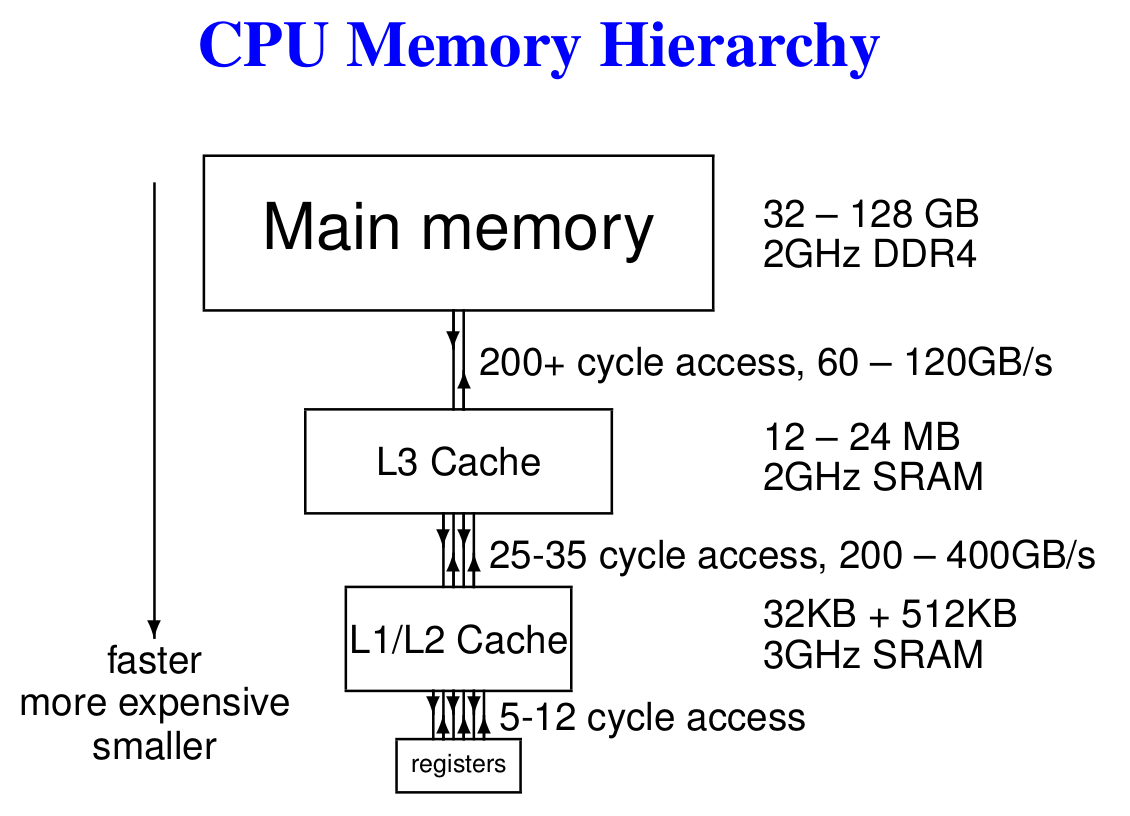
\includegraphics[width=11.0cm]{graphs/memory4.png}
\end{frame}
\subsection{Compute Capability}
\begin{frame}[fragile]
  \frametitle{GPU hardware: Compute Capability}
\begin{itemize}
\item {\color{mycolordef}Compute Capability} defines a set of features that the program can use
\item GPU cards are advertised to support particular compute capability
\item K80 has compute capability 3.7, while V100 is compute capability 7.0 and the latest Turing architecture supports 7.5
\item When you compile binary that would run on GPU, you specify on the features from what compute capability your code relies
\item You can also specify for what particular hardware you build the code and save binaries for different GPU cards in the same executable
\item Executable also contains so called {\color{mycolordef}PTX} code which is basically an assembler code for GPU hardware that supports the specified compute capability.
\item PTX allows {\color{mycolordef}JIT - just in time compilation}: if you try to run your binary on the card for which the code was not compiled it gets 
  recompiled at run time provided that the card is backward compatible
  with the specified compute capability.
\end{itemize}
\end{frame}

\subsection{Generations of GPU cards}
\begin{frame}[fragile]
  \frametitle{GPU hardware: Generations of GPU cards}
\begin{itemize}
\item For each compute capability NVIDIA releases many cards 
  for different usage mode: gaming, graphics, laptops, desktops, tablets, data center, etc
\item They differ by such hardware resources as memory, number of SMs, number of registers, etc.
\item We shall list here only several recent data center quality cards used for heavy computations. 

{\tiny
\begin{center}
\begin{tabular}{ |r|p{1.0cm}|p{0.9cm}|p{0.25cm}|r|p{0.7cm}|p{0.9cm}|p{0.8cm}|p{0.8cm}| } 
 \hline
 Model & {Micro Architecture} & {Compute Capability} & SMs  & cores &  Memory (GB) & {Connection to CPU} & {Bandwidth to CPU (GB/s)} & {Bandwidth to memory (GB/s)} \\ \hline
 K80   & Kepler               & 3.7                  & 2x13 & 2x2496& 2x12         & PCIe                & 12                        & 2x240                        \\ \hline
 P100  & Pascal               & 6.0                  & 56   & 3584  & 12, 16       & PCIe, NVlink        & 32, 160                   & 549, 732                     \\ \hline
 V100  & Volta                & 7.0                  & 80   & 5120  & 16, 32       & PCIe, NVlink        & 32, 300                   & 900                          \\ \hline
\end{tabular}
\end{center}
}

\item Modern consumer level GPU cards found in laptops and desktop typically can also be used for GPU computing.
\end{itemize}
\end{frame}
\subsection{Lab 1: Querying hardware}
\begin{frame}[fragile]
  \frametitle{GPU hardware: Lab 1: querying hardware}
\begin{itemize}
\item To find out how many GPU cards are there in a node, what kind, driver version, what processes are running on which GPU card, use {\color{mycolorcli}nvidia-smi}:
{\tiny
{\color{mycolorcli}
\begin{verbatim}
+-----------------------------------------------------------------------------+
| NVIDIA-SMI 410.72       Driver Version: 410.72       CUDA Version: 10.0     |
|-------------------------------+----------------------+----------------------+
| GPU  Name        Persistence-M| Bus-Id        Disp.A | Volatile Uncorr. ECC |
| Fan  Temp  Perf  Pwr:Usage/Cap|         Memory-Usage | GPU-Util  Compute M. |
|===============================+======================+======================|
|   0  Tesla K80           On   | 00000000:08:00.0 Off |                    0 |
| N/A   27C    P8    27W / 149W |      0MiB / 11441MiB |      0%      Default |
+-------------------------------+----------------------+----------------------+
|   1  Tesla K80           On   | 00000000:09:00.0 Off |                    0 |
| N/A   32C    P8    28W / 149W |      0MiB / 11441MiB |      0%      Default |
+-------------------------------+----------------------+----------------------+
|   2  Tesla K80           On   | 00000000:88:00.0 Off |                    0 |
| N/A   28C    P8    25W / 149W |      0MiB / 11441MiB |      0%      Default |
+-------------------------------+----------------------+----------------------+
|   3  Tesla K80           On   | 00000000:89:00.0 Off |                    0 |
| N/A   33C    P8    29W / 149W |      0MiB / 11441MiB |      0%      Default |
+-------------------------------+----------------------+----------------------+
                                                                               
+-----------------------------------------------------------------------------+
| Processes:                                                       GPU Memory |
|  GPU       PID   Type   Process name                             Usage      |
|=============================================================================|
|  No running processes found                                                 |
+-----------------------------------------------------------------------------+
\end{verbatim}
}
}

\end{itemize}
\end{frame}


\begin{frame}[fragile]
  \frametitle{GPU hardware: Lab 1: querying hardware}
\begin{itemize}
\item To submit a job in batch to gpu2 node that would run {\color{mycolorcli}nvidia-smi}:
{\color{mycolorcli}
\begin{verbatim}
cd cuda/labs/1
sbatch nvidia-smi.batch
\end{verbatim}
}
\item If we have enough GPUs, we can log into the node and use it interactively:
{\color{mycolorcli}
\begin{verbatim}
sinteractive -p gpu2 --gres=gpu:1 --reservation=CUDA
\end{verbatim}
}
\item Set up the environment {\color{mycolorcli}\verb|source cuda/labs/env.sh|} 
\item Above you ask for one gpu card in one gpu2 node. {\color{mycolorcli}\verb|--reservation|} only exists for the duration
  of this workshop. Otherwise, do not use it.

\item One can run {\color{mycolorcli}nvidia-smi} continously, every few seconds, as {\color{mycolorcli}top}, using {\color{mycolorcli}-l} flag. 
\item This can be very useful to diagnose problems: 
  \begin{itemize}
  \item is the program using too much GPU memory?
  \item is the load on GPU too low? 
  \item is there hardware problem with GPU?
  \end{itemize}
\end{itemize}
\end{frame}

\begin{frame}[fragile]
  \frametitle{GPU hardware: Lab 1: querying hardware}
\begin{itemize}
\item Note: one can restrict a program to see only some of the available GPUs by setting 
{\color{mycolorcli}\verb|CUDA_VISIBLE_DEVICES|} to the list of visible GPU cards, separated by comma
\item When you submit a job to SLURM scheduler, it sets this variable for you, so that each user on a node sees only as many GPU cards as was requested
\item Otherwise, the program sees all GPU cards and can grab them whether their are needed or not, possibly blocking other users
\end{itemize}
\end{frame}


\begin{frame}[fragile]
  \frametitle{GPU hardware: Lab 1: querying hardware}
\begin{itemize}
\item One can query the detailed parameters of the device with {\color{mycolorcli}deviceQuery} program that comes with CUDA.
\end{itemize}
{\tiny
{\color{mycolorcli}
\begin{verbatim}
/software/cuda-10.0-el7-x86_64/samples/1_Utilities/deviceQuery/deviceQuery Starting...

 CUDA Device Query (Runtime API) version (CUDART static linking)

Detected 1 CUDA Capable device(s)

Device 0: "Tesla K80"
  CUDA Driver Version / Runtime Version          10.0 / 10.0
  CUDA Capability Major/Minor version number:    3.7
  Total amount of global memory:                 11441 MBytes (11996954624 bytes)
  (13) Multiprocessors, (192) CUDA Cores/MP:     2496 CUDA Cores
  GPU Max Clock rate:                            824 MHz (0.82 GHz)
  Memory Clock rate:                             2505 Mhz
  Memory Bus Width:                              384-bit
  L2 Cache Size:                                 1572864 bytes
  Maximum Texture Dimension Size (x,y,z)         1D=(65536), 2D=(65536, 65536), 3D=(4096, 4096, 4096)
  Maximum Layered 1D Texture Size, (num) layers  1D=(16384), 2048 layers
  Maximum Layered 2D Texture Size, (num) layers  2D=(16384, 16384), 2048 layers
  Total amount of constant memory:               65536 bytes
  Total amount of shared memory per block:       49152 bytes
  Total number of registers available per block: 65536
  Warp size:                                     32
  Maximum number of threads per multiprocessor:  2048
  Maximum number of threads per block:           1024
...
\end{verbatim}
}
}

\end{frame}


\begin{frame}[fragile]
  \frametitle{GPU hardware: Lab 1: querying hardware}
{\tiny
{\color{mycolorcli}
\begin{verbatim}
...
  Max dimension size of a thread block (x,y,z): (1024, 1024, 64)
  Max dimension size of a grid size    (x,y,z): (2147483647, 65535, 65535)
  Maximum memory pitch:                          2147483647 bytes
  Texture alignment:                             512 bytes
  Concurrent copy and kernel execution:          Yes with 2 copy engine(s)
  Run time limit on kernels:                     No
  Integrated GPU sharing Host Memory:            No
  Support host page-locked memory mapping:       Yes
  Alignment requirement for Surfaces:            Yes
  Device has ECC support:                        Enabled
  Device supports Unified Addressing (UVA):      Yes
  Device supports Compute Preemption:            No
  Supports Cooperative Kernel Launch:            No
  Supports MultiDevice Co-op Kernel Launch:      No
  Device PCI Domain ID / Bus ID / location ID:   0 / 9 / 0
  Compute Mode:
     < Default (multiple host threads can use ::cudaSetDevice() with device simultaneously) >

deviceQuery, CUDA Driver = CUDART, CUDA Driver Version = 10.0, CUDA Runtime Version = 10.0, NumDevs = 1
Result = PASS

\end{verbatim}
}
}

\end{frame}


\section{CUDA programming}
\begin{frame}[fragile]
  \frametitle{CUDA programming}
\begin{itemize}
\item The native way to program GPU is to use \mydef{CUDA - Compute Unified Device Architecture} - from NVIDIA. 
\item The latest version of CUDA is 10.0
\item NVIDIA first was producing GPU cards as pure graphics accelerators before it was realized that GPU card can be used to speed up numerical computations, especially those that involve a lot of linear algebra
\item CUDA was introduced to support using GPU cards for numerical computations in 2007.
\item CUDA provides an extension of C/C++ syntax and libraries that allow to write functions, called {\color{mycolordef}kernels}, that get executed in parallel by multiple threads on GPU. 
\item CUDA allows to allocated/deallocate memory on GPU and copy data between CPU's RAM and GPU's global memory.
\item One can also program CUDA in Fortran, Python, Java.
\item Let us consider the simplest example of adding two vectors.
\end{itemize}
\end{frame}

\subsection{Lab 2: thread, block, grid, kernel}
\begin{frame}[fragile]
  \frametitle{CUDA programming: Lab 2: thread, block, grid, kernel}
\begin{itemize}
\item In this lab we are adding two vectors, {\color{mycolorcode}\verb|A|} and {\color{mycolorcode}\verb|B|}, 
  consisting of \verb|50000| floats. The result is put into {\color{mycolorcode}\verb|C|}.
\item Obviously different elements of the vectors can be added independently from each other in parallel.
\item First, in the main program we allocate memory for {\color{mycolorcode}\verb|A|}, 
  {\color{mycolorcode}\verb|B|}, {\color{mycolorcode}\verb|C|} 
  on the host as usual, with {\color{mycolorcode}\verb|malloc|}, and populate {\color{mycolorcode}\verb|A|} 
  and {\color{mycolorcode}\verb|B|} with random numbers.
\item Next we need to allocate memory on GPU card with {\color{mycolorcode}cudaMalloc}:
{\color{mycolorcode}
\begin{verbatim}
float *d_A = NULL, *d_B = NULL,  *d_C = NULL;
cudaMalloc((void **)&d_A, size);
cudaMalloc((void **)&d_B, size);
cudaMalloc((void **)&d_C, size);
\end{verbatim}
}

\end{itemize}
\end{frame}


\begin{frame}[fragile]
  \frametitle{CUDA programming: Lab 2: thread, block, grid, kernel}
\begin{itemize}
\item Copy data from the host to the device:
{\color{mycolorcode}
\begin{verbatim}
cudaMemcpy(d_A, h_A, size, cudaMemcpyHostToDevice);
cudaMemcpy(d_B, h_B, size, cudaMemcpyHostToDevice);
\end{verbatim}
}
\item Next we need to decide how to divide our work into blocks of threads.
  \begin{itemize}
  \item Each block runs entirely on one of SMs. 
  \item Different blocks might run in parallel or sequentially and get launched in any order on the same or different SMs.
  \item Each block can have no more than 1024 threads.
  \item Since the warp size is 32, block size should be divisible by 32.
  \end{itemize}
\item We shall consider tradeoffs for different choices later but for now let us just use 
  256 threads per block and compute how many blocks we need in order to add 50000 elements.
{\tiny
{\color{mycolorcode}
\begin{verbatim}
int numElements = 50000;
int threadsPerBlock = 256;
int blocksPerGrid =(numElements + threadsPerBlock - 1) / threadsPerBlock;
\end{verbatim}
}
}
\end{itemize}
\end{frame}


\begin{frame}[fragile]
  \frametitle{CUDA programming: Lab 2: thread, block, grid, kernel}
\begin{itemize}
\item The actual work is done in a {\color{mycolordef}kernel} - function executed by each thread in the job:
{\tiny
{\color{mycolorcode}
\begin{verbatim}
__global__ void vectorAdd(const float *A, const float *B, float *C, int numElements)
{
    int i = blockDim.x * blockIdx.x + threadIdx.x;
    if (i < numElements)
        C[i] = A[i] + B[i];
}
\end{verbatim}
}
}
\item Notice {\color{mycolorcode}\verb|__global__|} in front of the GPU function
\item From inside the kernel one can use the following variables:
  \begin{itemize}
    \item {\color{mycolorcode}\verb|blockDim.x|} - block size;
    \item {\color{mycolorcode}\verb|blockIdx.x|} - block id in the grid;
    \item {\color{mycolorcode}\verb|threadIdx.x|} - thread id in the block;
  \end{itemize}
\item For each thread, the kernel computes the index {\color{mycolorcode}\verb|i|} of the vector variables that it handles.
\item The corresponding elements of {\color{mycolorcode}\verb|A|} and {\color{mycolorcode}\verb|B|} are added and stored in {\color{mycolorcode}\verb|C|}.
\item There might be more threads than the number of elements to add, therefore {\color{mycolorcode}\verb|if|} is needed.
\end{itemize}
\end{frame}

\begin{frame}[fragile]
  \frametitle{CUDA programming: Lab 2: thread, block, grid, kernel}
\begin{itemize}
\item To call the kernel from the host program, one must specify the number of blocks and threads per block:
{\tiny
{\color{mycolorcode}
\begin{verbatim}
vectorAdd<<<blocksPerGrid, threadsPerBlock>>>(d_A, d_B, d_C, numElements);
\end{verbatim}
}
}
\item The same kernel can be called with different grid and block dimensions.
\item After the kernel completes, we copy the result back to the host and free device memory:
{\color{mycolorcode}
\begin{verbatim}
cudaMemcpy(h_C, d_C, size, cudaMemcpyDeviceToHost);
cudaFree(d_A);
cudaFree(d_B);
cudaFree(d_C);
\end{verbatim}
}
\item Finally we free memory for host variables.
\end{itemize}
\end{frame}


\begin{frame}[fragile]
  \frametitle{CUDA programming: Lab 2: thread, block, grid, kernel}
\begin{itemize}
\item Until compute capability 5.0, the device code should be in the same file as the host code that calls the kernel.
\item Since we are using K80 with compute cability 3.7, this is the case for us.
\item The files that contain device code typically have {\color{mycolorcli}cu} extension.
\item To compile the code, we need to use {\color{mycolorcli}nvcc} compiler that would compile device code and call system compiler to build the host code and then link them together:
{\color{mycolorcli}
\begin{verbatim}
nvcc -o vectorAdd vectorAdd.cu
\end{verbatim}
}
\item By default, {\color{mycolorcli}nvcc} would compile the code for the current hardware. One can specify compute capability and exact SM architecture, one can even specify several. 
JIT compilation is supported as well to be able to run on new hardware for which the program was not originally compiled. 

\end{itemize}
\end{frame}


\begin{frame}[fragile]
  \frametitle{CUDA programming: Lab 2: thread, block, grid, kernel}
\begin{itemize}
\item Now when we understood the overall structure of {\color{mycolorcli}\verb|vectorAdd.cu|}, let us look at the original file from {\color{mycolorcli}\verb|samples/0_Simple/vectorAdd|}
\item The main thing that I skipped for simplicity is error handling.
{\tiny
{\color{mycolorcli}
\begin{verbatim}
cudaError_t err = cudaSuccess;
...
err = cudaMalloc((void **)&d_A, size);
if (err != cudaSuccess)
    {
        fprintf(stderr, "Failed to allocate device vector A (error code %s)!\n", 
                cudaGetErrorString(err));
        exit(EXIT_FAILURE);
    }
...
err = cudaMemcpy(d_A, h_A, size, cudaMemcpyHostToDevice);
...
vectorAdd<<<blocksPerGrid, threadsPerBlock>>>(d_A, d_B, d_C, numElements);
err = cudaGetLastError();
...
err = cudaFree(d_A);
\end{verbatim}
}
}
\item The error checking should be done after each CUDA call. Otherwise, you might not notice that the program is working incorrectly and producing wrong results.
\end{itemize}
\end{frame}


\subsection{Lab 3: shared memory, barrier}
\begin{frame}[fragile]
  \frametitle{CUDA programming: shared memory, barrier}
\begin{itemize}
\item First let us implement straightforward matrix multiplication ({\color{mycolorcli}matrixMul0.cu})
  and then reimplement it using shared  memory ({\color{mycolorcli}matrixMul1.cu}) and compare performance between two GPU and CPU sequential implementations.
\item We define \mycode{Matrix} structure as follows:
{\color{mycolorcode}
\begin{verbatim}
typedef struct
{
  int width;
  int height;
  float * elements;
} Matrix;
\end{verbatim}
}
\item We allocate memory for matrices \mycode{A}, \mycode{B}, \mycode{C} on the host and device, generate random elements for \mycode{A} and \mycode{B} on the host and copy them to the device.
\end{itemize}
\end{frame}

\begin{frame}[fragile]
  \frametitle{CUDA programming: shared memory, barrier}
\begin{itemize}
\item To measure the timing for different kernels, we use cuda events:

{\color{mycolorcode}
\begin{verbatim}
cudaEvent_t start, stop;
cudaEventCreate(&start);
cudaEventCreate(&stop);
cudaEventRecord(start);

MatMulKernel<<<dimGrid, dimBlock>>>(d_A, d_B, d_C);

cudaEventRecord(stop);
cudaEventSynchronize(stop);
float milliseconds = 0;
cudaEventElapsedTime(&milliseconds, start, stop);
\end{verbatim}
}

\item In general, cuda events can be used to synchronize various threads.

\end{itemize}
\end{frame}

\begin{frame}[fragile]
  \frametitle{CUDA programming: shared memory, barrier}
\begin{itemize}
\item Notice that grids and blocks in CUDA can be 1-, 2-, 3-dimensional.
\item To multiply 2D matrices, it is natural to use 2D grids and blocks.
\item When calling a kernel, instead of 1D integers for grid and block sizes, 
  one can use 3D tuples of type \mycode{dim3}, in which by default, if not specified, all three components are set to 1:
{\color{mycolorcode}
\begin{verbatim}
dim3 dimBlock(BLOCK_SIZE, BLOCK_SIZE);
dim3 dimGrid(B.width/dimBlock.x, A.height/dimBlock.y);
...
MatMulKernel<<<dimGrid, dimBlock>>>(d_A, d_B, d_C);
\end{verbatim}
}
\end{itemize}
\end{frame}

\begin{frame}[fragile]
  \frametitle{CUDA programming: shared memory, barrier}
\begin{itemize}
\item In the first GPU implementation of matrix multiplication, we let each thread to 
  compute a separate entry of \mycode{C} matrix:
{\color{mycolorcode}
\begin{verbatim}
__global__ void MatMulKernel(Matrix A, Matrix B, Matrix C)
{
  float Cvalue = 0;
  int row = blockIdx.y * blockDim.y + threadIdx.y;
  int col = blockIdx.x * blockDim.x + threadIdx.x;
  for (int e = 0; e < A.width; ++e)
    Cvalue += A.elements[row * A.width + e] * 
              B.elements[e * B.width + col];
  C.elements[row * C.width + col] = Cvalue;
}
\end{verbatim}
}
\item Notice that \mycode{blockIdx}, \mycode{blockDim}, \mycode{threadIdx} are of type \mycode{dim3}
\end{itemize}
\end{frame}

\begin{frame}[fragile]
  \frametitle{CUDA programming: shared memory, barrier}
\begin{itemize}
\item We compare the performance of CUDA program with the performance of a single threaded straightforward matrix multiplication on CPU:
{\tiny
{\color{mycolorcode}
\begin{verbatim}
void sequential_cpu(Matrix A, Matrix B, Matrix C)
{
  for(int i = 0; i < C.height; ++i)
    {
      for(int j = 0; j < C.width; ++j)
        {
          C.elements[i*C.width + j] = 0;
          for(int ac = 0; ac < A.width; ++ac)
            {
              for(int br = 0; br < B.height; ++br)
                {
                  C.elements[i*C.width + j] += 
                    A.elements[i*A.width + ac] * 
                    B.elements[j + br*B.width];
                }
            }
        }
    }
}
\end{verbatim}
}
}
\item To multiply $160x240$ and $240x320$ matrices took $0.4$ ms with GPU implementation on K80 and $14320$ ms on a single Broadwell CPU core of \mycli{gpu2} partition. 
  Naive GPU implementation on a 4 year old K80 is $35800$ times faster!
\end{itemize}
\end{frame}

\begin{frame}[fragile]
  \frametitle{CUDA programming: shared memory, barrier}
\begin{itemize}
\item Notice: the first time the kernel runs on GPU in your program, it is slower than in subsequent times (0.6 ms vs 0.4 ms for this problem) due to some warming up overhead.
\item To take this into account, the kernel was called 5 times and the results are averaged over the last 4 measurements.
\item In this GPU implementation each element of \mycode{A} is read \mycode{B.width} times and each element of 
  \mycode{B} is read \mycode{A.height} times from global memory. 
\item Since global memory is slow, in ideal we want to read things from there only
  once and cache it in \mydef{shared memory} which is much faster. 
\item In ideal it would also be best to read data from global memory in a \mydef{coalesced} way to take advantage of automatic \mydef{caching} in L1, L2 caches:
  \begin{itemize}
    \item When you ask to read data at address \mycode{A} of size, say 4 bytes, instead hardware would read a \mydef{cacheline} of something like 32 of such elements and store them in fast but small cache.
    \item If the next address you read is available from cache, it is taken from there and global memory is not read
  \end{itemize}
\end{itemize}
\end{frame}


\begin{frame}[fragile]
  \frametitle{CUDA programming: shared memory, barrier}
\begin{itemize}
\item In the second implementation of matrix multiplication we shall divide each matrix into submatrices of $16x16$ size
\item Each thread block caches submatrix of \mycode{A} 
  and submatrix of \mycode{B} in shared memory before performing 
  a straightforward matrix multiplication of such submatrices.
\item As a result, each element of \mycode{A} is accessed {\color{mycolorcode}\verb|B.width/16|} 
  times and each element of \mycode{B} is accessed {\color{mycolorcode}\verb|A.height/16|} 
  times reducing the load on the global memory by a factor of $256$.
\end{itemize}
\end{frame}

\begin{frame}[fragile]
  \frametitle{CUDA programming: shared memory, barrier}
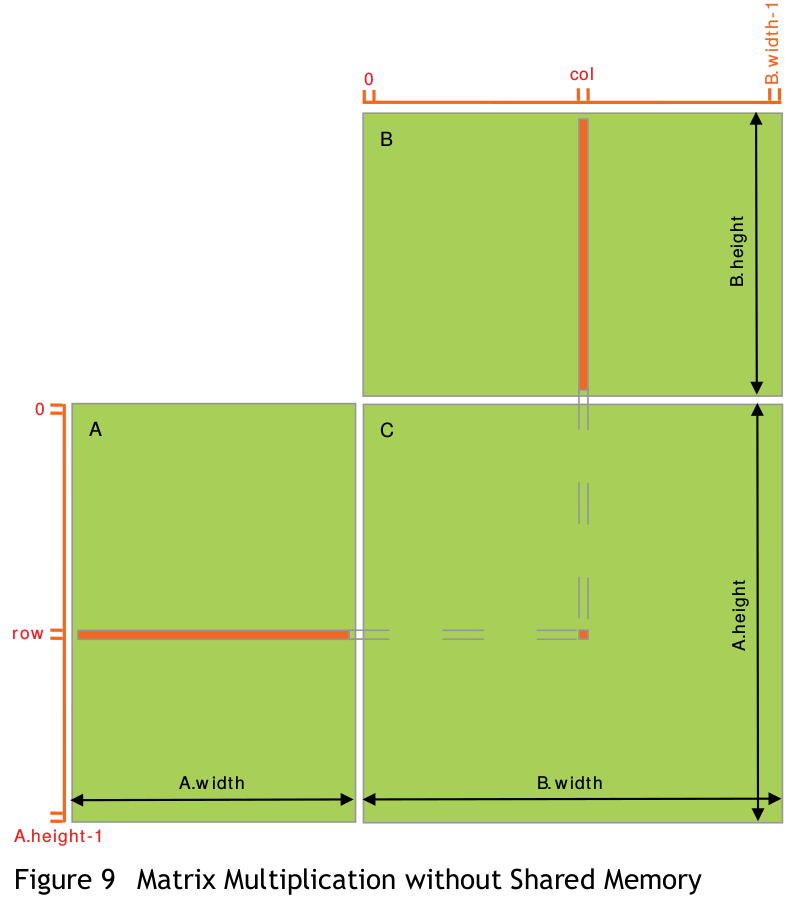
\includegraphics[width=5.5cm]{graphs/matMult1.png}
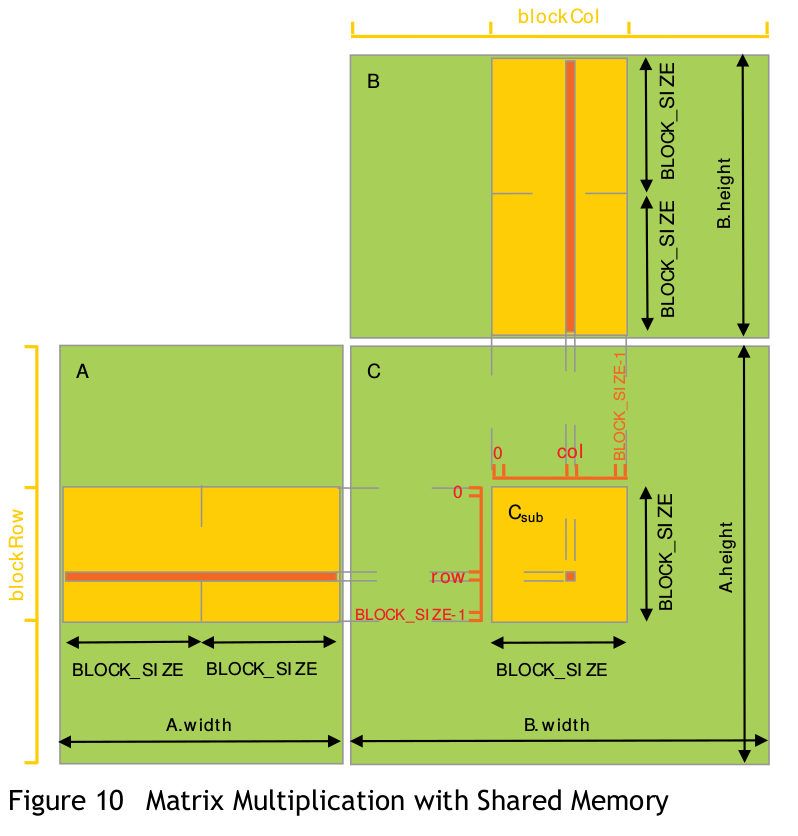
\includegraphics[width=5.5cm]{graphs/matMult2.png}
\end{frame}

\begin{frame}[fragile]
  \frametitle{CUDA programming: shared memory, barrier}
  \begin{itemize}
  \item To deal with submatrices, we need to modify the definition of the \mycode{Matrix} structure:
    {\color{mycolorcode}
      {\tiny
\begin{verbatim}
typedef struct
{
  int width;
  int height;
  int stride;
  float * elements;
} Matrix;
\end{verbatim}
      }
    }
  \item Here \mycode{width} refers to the width of the submatrix while \mycode{stride} refers to the width of the big matrix.
  \item Same structure can be used for the big matrix: 
    \begin{itemize}
    \item in that case \mycode{width = stride}.
    \end{itemize}
  \item The big matrix is subdivided into submatrices because you can store only so much in shared memory. For K80, it is up to 48kb.
  \end{itemize}
\end{frame}

\begin{frame}[fragile]
  \frametitle{CUDA programming: shared memory, barrier}
  \begin{itemize}
  \item We define several convenience device functions:
    \begin{itemize}
    \item to extract a submatrix in place:
      {\color{mycolorcode}
        {\tiny
\begin{verbatim}
__device__ Matrix GetSubMatrix(Matrix A, int row, int col)
{
  Matrix Asub;
  Asub.width = BLOCK_SIZE;
  Asub.height = BLOCK_SIZE;
  Asub.stride = A.stride;
  Asub.elements = &A.elements[A.stride * BLOCK_SIZE * row + 
                              BLOCK_SIZE * col];
  return Asub;
}
\end{verbatim}
      }
    }
    \item to get/set matrix element:
      {\color{mycolorcode}
        {\tiny
\begin{verbatim}
__device__ float GetElement(const Matrix A, int row, int col)
{
  return A.elements[row * A.stride + col];
}

__device__ void SetElement(Matrix A, int row, int col, float value)
{
  A.elements[row * A.stride + col] = value;
}
\end{verbatim}
      }
    }
    \end{itemize}
  \item Notice the above device functions are called from the GPU kernel that does the main job
  \end{itemize}
\end{frame}

\begin{frame}[fragile]
  \frametitle{CUDA programming: shared memory, barrier}
  \begin{itemize}
  \item Until compute capability 3.5, CUDA 5.0, only host could call a function that runs on GPU
  \item Now GPU functions can call GPU functions
  \item This feature is called \mydef{dynamic parallelism} and it  allows implementing, for example, recursive algorithms on GPU
  \item In the main kernel, each block computes a submatrix \mycode{Csub} by looping over submatrices \mycode{Asub} and \mycode{Bsub}
  \item Each submatrix is copied from the global memory into the shared memory
  \item All threads in a block wait on a \mydef{barrier} {\color{mycolorcode}\verb| __syncthreads()|} to make sure that all the necessary entries are loaded into shared memory
    before using them.
  \item Another barrier is inserted at the end of the loop iteration to make sure that all the threads in a block finished using shared memory before overwriting it with new submatrices
  \end{itemize}
\end{frame}

\begin{frame}[fragile]
  \frametitle{CUDA programming: shared memory, barrier}
{\tiny
{\color{mycolorcode}
\begin{verbatim}
__global__ void MatMulKernel(Matrix A, Matrix B, Matrix C)
{
  int blockRow = blockIdx.y;
  int blockCol = blockIdx.x;

  // Each thread block computes one sub-matrix Csub of C
  Matrix Csub = GetSubMatrix(C, blockRow, blockCol);

  // Each thread computes one element of Csub
  // by accumulating results into Cvalue
  float Cvalue = 0;

  int row = threadIdx.y;
  int col = threadIdx.x;

  // Loop over all the sub-matrices of A and B that are required to compute Csub
  // Multiply each pair of sub-matrices together
  // and accumulate the results
  for(int m = 0; m < (A.width/BLOCK_SIZE); ++m)
    {
      // Get sub-matrix Asub of A
      Matrix Asub = GetSubMatrix(A, blockRow, m);
      
      // Get sub-matrix Bsub of B
      Matrix Bsub = GetSubMatrix(B, m, blockCol);
\end{verbatim}
}
}
\end{frame}


\begin{frame}[fragile]
  \frametitle{CUDA programming: shared memory, barrier}
{\tiny
{\color{mycolorcode}
\begin{verbatim}
      // Shared memory used to store Asub and Bsub respectively
      __shared__ float As[BLOCK_SIZE][BLOCK_SIZE];
      __shared__ float Bs[BLOCK_SIZE][BLOCK_SIZE];

      // Load Asub and Bsub from device memory to shared memory
      // Each thread loads one element of each sub-matrix
      As[row][col] = GetElement(Asub, row, col);
      Bs[row][col] = GetElement(Bsub, row, col);

      // Synchronize to make sure the sub-matrices are loaded
      // before starting the computation

      __syncthreads();
      // Multiply Asub and Bsub together
      for(int e = 0; e < BLOCK_SIZE; ++e)
        {
          Cvalue += As[row][e] * Bs[e][col];
        }

      // Synchronize to make sure that the preceding
      // computation is done before load two new sub-matrices of A and B in the next
      // iteration
      __syncthreads();
    }
  // Write Csub to device memory
  // Each thread writes one element
  SetElement(Csub, row, col, Cvalue);
}

\end{verbatim}
}
}
\end{frame}


\begin{frame}[fragile]
  \frametitle{CUDA programming: shared memory, barrier}
\begin{itemize}
\item By using shared memory we further speed up the program by another factor of $2.5$: it now takes $0.16$ ms for the same matrices.
\item Trying to multiply big matrices on a single CPU core takes forever. 
\item Of course, on CPU one can also parallelize the program and take advantage of vectorization
\item There are 28 CPU cores on midway2 nodes
\item Vectorization might also give another factor of 16 or so
\item Still: to parallelize on CPU also requires some efforts (probably using OpenMP) and the expected performance gain would probably be 10-30 times worse than on K80.
\item Of course, this was just an excercise. To do linear algebra in your application, you should use libraries:
  \begin{itemize}
  \item on CPU: MKL, OpenBlas, Atlas, Plasma, Eigen, SuperLU...
  \item on GPU: cuBLAS, cuSPARSE, Magma...
  \end{itemize}
\end{itemize}
\end{frame}


\subsection{Lab 4: intrinsics, streams, tools}
\begin{frame}[fragile]
  \frametitle{CUDA programming: Lab 4: intrinsics, streams, tools}
\begin{itemize}
\item In this lab we shall learn about \mydef{CUDA math library}, \mydef{streams}, \mydef{nsight} tools
\item Let us create on CPU a big array, initialize it with random numbers, copy it to GPU, apply some math functions to it and copy it back to the host.
\item Here is the kernel
{\tiny
{\color{mycolorcode}
\begin{verbatim}
__global__ void map(float *d_a, int n, int m)
{
  int id = blockDim.x * blockIdx.x  + threadIdx.x;
  
  if(id < n)
    for(int i = 0; i < m; ++i)
      {
        d_a[id] = sinf(d_a[id]) + cosf(d_a[id]);
        d_a[id] = expf(d_a[id]);
        d_a[id] = rsqrtf(d_a[id]) - d_a[id];
      }
}
\end{verbatim}
}
}
\item In CUDA there are \mydef{standard math functions} - can be executed both on the host and device -  and \mydef{intrinsic functions} - can only run on device, are faster but less precise.
\item The code above uses standard functions.
\end{itemize}
\end{frame}

\begin{frame}[fragile]
  \frametitle{CUDA programming: Lab 4: intrinsics, streams, tools}
\begin{itemize}
\item Examples of standard math functions: \mycode{sqrtf}, \mycode{sqrt}, \mycode{rsqrtf}, \mycode{rsqrt}, \mycode{sinf}, \mycode{sin}, etc. Those are single and double precision functions.
\item Examples of the corresponding intrisic functions: {\color{mycolorcode}\verb|__fsqrt_rn|}, {\color{mycolorcode}\verb|__frsqrt_rn|}, {\color{mycolorcode}\verb|__sinf|}, etc. The precision is less than float.
\item If one can afford less accurate functions, one can either replace the functions in the code or use compile option {\color{mycolorcli}\verb|--use_fast_math|} to replace all the standard functions by the corresponding intrinsic 
  functions.
\item Let us measure the performance of the same kernel with standard and intrinsic math functions: 131 vs 27 ms! This kernel runs almost 5 times faster with intrinsic functions than with standard ones.
\item Let us look how the results are different:
{\tiny
{\color{mycolorcli}
\begin{verbatim}
a[0] = 1.74003, a[1] = 1.45576, a[2] = -3.50318, a[3] = -3.0294, a[4] = -3.22013 ...
vs
a[0] = 1.74017, a[1] = 1.45575, a[2] = -3.50318, a[3] = -3.02938, a[4] = -3.22022 ...
\end{verbatim}
}
}
\item Not a big difference in numerical results.
\item Consult the tables in the ``CUDA C Programming Guide'' for precision guarantees and the complete list of the available functions.
\end{itemize}
\end{frame}


\begin{frame}[fragile]
  \frametitle{CUDA programming: Lab 4: intrinsics, streams, tools}
\begin{itemize}
\item Let us run the program through \mydef{nvvp profiler}
\item We see that first the program spends significant time transfering data from host to device, then comparable amount of time is spent on the computations and transfering the results back to the host.
\end{itemize}
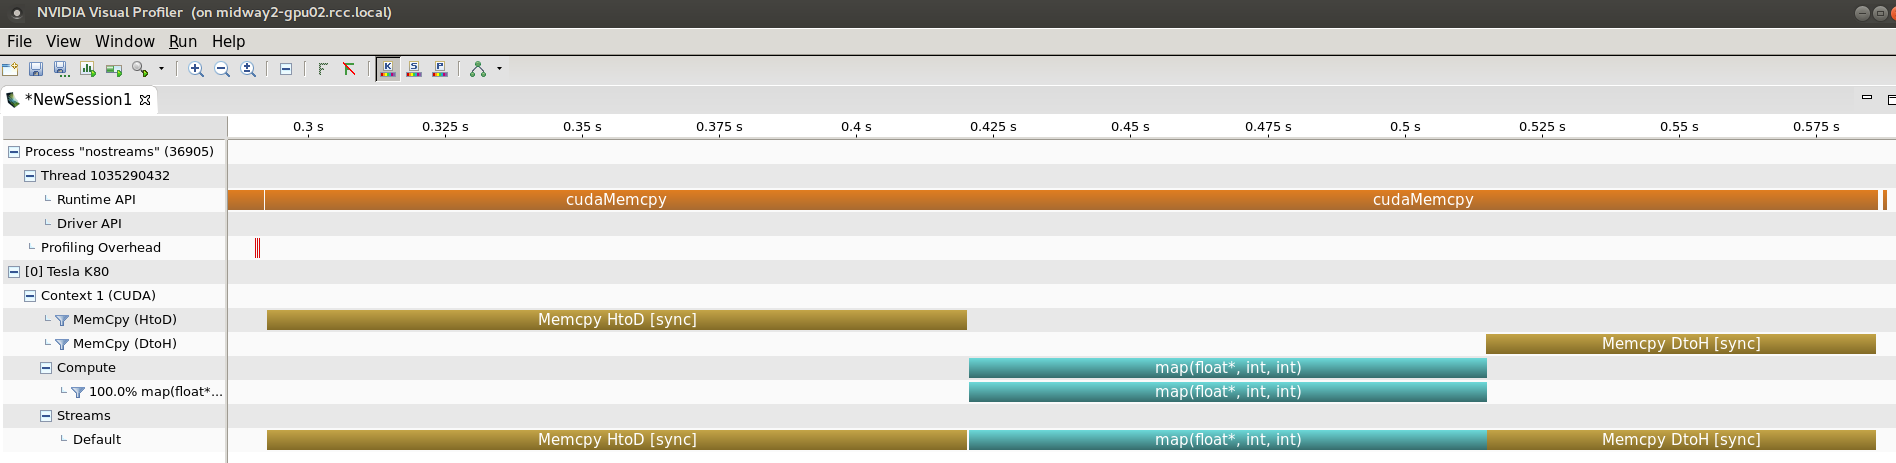
\includegraphics[width=11.9cm]{graphs/nostreams.png}
\begin{itemize}
\item Meanwhile, the computations are embarrasingly parallel and independent for each element of the array.
\item Would not it be better first to transfer a part of data, start computations on GPU on the first part of the data, transfer in parallel with the computations second part, etc. to hide the latency
\end{itemize}
\end{frame}

\begin{frame}[fragile]
  \frametitle{CUDA programming: Lab 4: intrinsics, streams, tools}
\begin{itemize}
\item Some devices of compute capability 2.x and higher can execute multiple
kernels concurrently. Applications may query this capability by checking the
\mycli{concurrentKernels} device property, which is equal to 1 for
devices that support it.
\item The maximum number of kernel launches that a device can execute concurrently
depends on its compute capability.
\item Some devices can perform an asynchronous memory copy to or from the GPU
concurrently with kernel execution. Applications may query this capability by checking
the \mycli{asyncEngineCount} device property, which is greater
than zero for devices that support it. If host memory is involved in the copy, it must be
page-locked
\item Some devices of compute capability 2.x and higher can overlap copies to and from the
device. Applications may query this capability by checking the \mycli{asyncEngineCount}
device property, which is equal to 2 for devices that support
it. In order to be overlapped, any host memory involved in the transfers must be page-locked.

\end{itemize}
\end{frame}


\begin{frame}[fragile]
  \frametitle{CUDA programming: Lab 4: intrinsics, streams, tools}
\begin{itemize}
\item For K80, according to \mycli{deviceQuery} from Lab 1:
{\tiny
{\color{mycolorcli}
\begin{verbatim}
Concurrent copy and kernel execution:  Yes with 2 copy engine(s)
\end{verbatim}
}
}
\item CUDA construction that can help to interleave computations and data transfer is called \mydef{streams}
\item A stream is a sequence of commands (possibly issued by different host threads) that
execute in order. Different streams, on the other hand, may execute their commands out
of order with respect to one another or concurrently.
\item A stream is defined by creating a stream object and specifying it as the stream parameter
to a sequence of kernel launches and host to/from device memory copies.
\item To use streams for data transfer between host and device, one needs to allocated memory on the host not with \mycode{malloc} but as follows
{\color{mycolorcode}
\begin{verbatim}
 float *h_a = NULL;
  cudaMallocHost(&h_a, size);
\end{verbatim}
}
to ensure that the memory allocated on the host is \mydef{page-locked} (cannot be swapped)
\end{itemize}
\end{frame}


\begin{frame}[fragile]
  \frametitle{CUDA programming: Lab 4: intrinsics, streams, tools}
\begin{itemize}
\item Next we need to create streams:
{\color{mycolorcode}
\begin{verbatim}
cudaStream_t stream[nstreams];
for(int i = 0; i < nstreams; ++i)
  cudaStreamCreate(&stream[i]);
\end{verbatim}
}
\item Send data between host and device in batches and run a kernel on each batch to interleave computations and data transfer:
{\tiny
{\color{mycolorcode}
\begin{verbatim}
for(int i = 0; i < nstreams; ++i)
{
  cudaMemcpyAsync(d_a + i*batch, h_a + i*batch, batch_size, cudaMemcpyHostToDevice, stream[i]);
  map<<<grid_size, block_size, 0, stream[i]>>>(d_a + i*batch, batch, iterations)
  cudaMemcpyAsync(h_a + i*batch, d_a + i*batch, batch_size, cudaMemcpyDeviceToHost, stream[i]);
}
\end{verbatim}
}
}
\item Notice: we provide \mycode{stream[i]} argument to data transfer operations and to a kernel call.
\item Also note: instead of \mycode{cudaMemcpy} we use asynchronous version \mycode{cudaMemcpyAsync} that, contrary to \mycode{cudaMemcpy} immediately returns without waiting for data transfer to finish.
\end{itemize}
\end{frame}

\begin{frame}[fragile]
  \frametitle{CUDA programming: Lab 4: intrinsics, streams, tools}
\begin{itemize}
\item To free resources, we need to destroy streams and release page-locked memory (not with \mycode{free} but with \mycode{cudaFreeHost}):
{\color{mycolorcode}
\begin{verbatim}
for(int i = 0; i < nstreams; ++i)
  cudaStreamDestroy(streams[i])
cudaFreeHost(h_a);
\end{verbatim}
}
\item In case the device is still doing work in the stream when \mycode{cudaStreamDestroy()} is
called, the function will return immediately and the resources associated with the stream
will be released automatically once the device has completed all work in the stream.
\item Kernel launches and host to/from device memory copies that do not specify any stream
parameter, or equivalently that set the stream parameter to zero, are issued to the default
stream. They are therefore executed in order.
\end{itemize}
\end{frame}


\begin{frame}[fragile]
  \frametitle{CUDA programming: Lab 4: intrinsics, streams, tools}
\begin{itemize}
\item Let us now run nvvp and see if we succeeded in interleaving data transfer and computations:
\end{itemize}
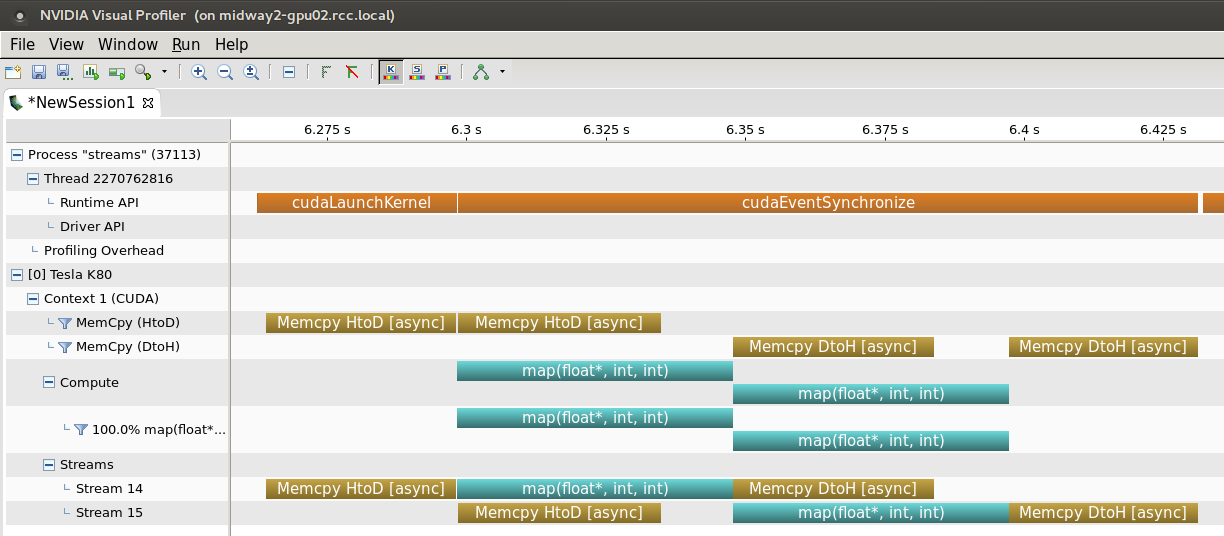
\includegraphics[width=11.9cm]{graphs/streams.png}
\end{frame}

\begin{frame}[fragile]
  \frametitle{CUDA programming: Lab 4: intrinsics, streams, tools}
\begin{itemize}
\item As you can see, kernel and data transfer are indeed interleaved but only one kernel runs at a time. This is probably the limitation of K80.
\item Let us see how it affected timing: 223 ms vs 138 ms.
\item Newer GPU cards might benefit more from streams.
\item There are various ways to explicitly synchronize streams with each other:
  \begin{itemize}
  \item \mycode{cudaDeviceSynchronize()} waits until all preceding commands in all streams of all
    host threads have completed.
  \item \mycode{cudaStreamSynchronize()} takes a stream as a parameter and waits until all preceding
    commands in the given stream have completed. It can be used to synchronize the host
    with a specific stream, allowing other streams to continue executing on the device.
  \item \mycode{cudaStreamWaitEvent()} takes a stream and an event as parameters and makes all the commands added to the given stream after
    the call to \mycode{cudaStreamWaitEvent()} delay their execution until the given event has
    completed. The stream can be 0, in which case all the commands added to any stream
    after the call to \mycode{cudaStreamWaitEvent()} wait on the event.
  \end{itemize}
\end{itemize}
\end{frame}

\begin{frame}[fragile]
  \frametitle{CUDA programming: Lab 4: intrinsics, streams, tools}
\begin{itemize}
\item More ways to explicitly synchronize streams with each other.
  \begin{itemize}
  \item \mycode{cudaStreamQuery()} provides applications with a way to know if all preceding
    commands in a stream have completed
  \end{itemize}
  \item One can insert a \mydef{callback} at any point into a stream via
    \mycode{cudaStreamAddCallback()}. A callback is a function that is executed on the host once
    all commands issued to the stream before the callback have completed. Callbacks in
    stream 0 are executed once all preceding tasks and commands issued in all streams
    before the callback have completed.
  \item The relative priorities of streams can be specified at creation using
    \mycode{cudaStreamCreateWithPriority()}.
\end{itemize}
\end{frame}

\begin{frame}[fragile]
  \frametitle{CUDA programming: Lab 4: intrinsics, streams, tools}
\begin{itemize}
  \item Instead of specifying what tasks run in what streams and what are dependencies between the tasks, one can use \mydef{graphs}
  \item Graphs present a new model for work submission in CUDA. A graph is a series of
    operations, such as kernel launches, connected by dependencies, which is defined
    separately from its execution. 
  \item This allows a graph to be defined once and then launched
    repeatedly. 
  \item Separating out the definition of a graph from its execution enables a number
    of optimizations: first, CPU launch costs are reduced compared to streams, because
    much of the setup is done in advance; second, presenting the whole workflow to CUDA
    enables optimizations which might not be possible with the piecewise work submission
    mechanism of streams.
  \item Graphs can be created with Graph API or by capturing an old fashioned streams based program.
\end{itemize}
\end{frame}


\begin{frame}[fragile]
  \frametitle{CUDA programming: Lab 4: intrinsics, streams, tools}
\begin{itemize}
\item As was mentioned before, to interleave data transfer and computations, the corresponding part of the host memory should be \mydef{pinned} or \mydef{page-locked}.
\item That means that it cannot be swapped to disk by OS.
\item Other uses of pinned memory:
  \begin{itemize}
  \item On some devices, page-locked host memory can be mapped into the address space
    of the device, eliminating the need to copy it to or from device memory
  \item On some systems bandwidth between host memory and device
    memory is higher if host memory is allocated as page-locked
  \end{itemize}
\item However, page-locked host memory is a scarce resource, so allocations in page-locked
  memory will start failing long before allocations in pageable memory. In addition, by
  reducing the amount of physical memory available to the operating system for paging,
  consuming too much page-locked memory reduces overall system performance.
\end{itemize}
\end{frame}

\begin{frame}[fragile]
  \frametitle{CUDA programming: Lab 4: intrinsics, streams, tools}
\begin{itemize}
\item We have already seen \mycli{nvvp} profiler.
\item CUDA comes with a suite of tools for debugging and profiling:
  \begin{itemize}
  \item There IDE with debugger, profiler, editor called \mycli{nsight}
  \item For \mycli{nsight} to show the source code, you need to compile it with \mycli{-g -G} option to \mycli{nvcc}
  \item Instead of using \mycli{nsight} GUI, you can run cli-based \mycli{cuda-gdb} which has similar interface as \mycli{gdb}. It allows to look into each thread separately.
  \item \mycli{cuda-memcheck} can be used to diagnose memory problems
  \item If you cannot run profiler on the node interactively, you can run it as a batch job and then look at the results with GUI.
  \item You can also run \mycli{nsight} remotely
  \end{itemize}
\item \mycli{nsight} is supposed to be deprecated soon and replaced by \mycli{nsight compute} and \mycli{nsight systems}. So far I can run those on my laptop (Ubuntu 16.04) but not on midway (Scientific Linux 7): they seem to require newer version of \mycli{glibc}.
\end{itemize}
\end{frame}


\begin{frame}[fragile]
  \frametitle{CUDA programming: Lab 4: intrinsics, streams, tools}
\begin{itemize}
\item We have already seen how to use \mydef{events} to time program execution.
\item CUDA lets the application asynchronously record events at
  any point in the program and query when these events are completed. 
\item An event has completed when all tasks - or optionally, all commands in a given stream - preceding the
  event have completed. 
\item Events in stream zero are completed after all preceding tasks and
  commands in all streams are completed.
\end{itemize}
{\small
{\color{mycolorcode}
\begin{verbatim}
cudaEvent_t start, stop;
cudaEventCreate(&start); cudaEventCreate(&stop);
cudaEventRecord(start);
map<<<grid_size, block_size>>>(d_a, N, iterations);
cudaEventRecord(stop); 
cudaEventSynchronize(stop);
cudaEventElapsedTime(&milliseconds, start, stop);
cudaEventDestroy(start); cudaEventDestroy(stop);
\end{verbatim}
}
}
\end{frame}


\subsection{Lab 5: occupancy, libraries}
\begin{frame}[fragile]
  \frametitle{CUDA programming: Lab 5: occupancy, libraries}
\begin{itemize}
\item In this lab we investigate how to select block size for optimal performance.
\item First we randomly generate couple arrays directly on GPU using \mycode{curand} library:
\end{itemize}
\begin{columns}
\begin{column}{0.55\textwidth}
{\tiny
{\color{mycolorcode}
\begin{verbatim}
#include <iostream>
#include <curand.h>
using namespace std;

struct random_d_array
{
  float *data;
  int n;

  random_d_array(int n) :n{n}
  {
    cudaMalloc((void**)&data, n*sizeof(float));
    curandGenerator_t gen;
    curandCreateGenerator(&gen, CURAND_RNG_PSEUDO_DEFAULT);
    curandGenerateUniform(gen, data, n);
  }
  
  ~random_d_array()
  {
    cudaFree(&data);
  }
};

\end{verbatim}
}
}
\end{column}
\begin{column}{0.45\textwidth}

\begin{itemize}
\item At compilation the code needs to be linked with the library:
{\tiny
{\color{mycolorcli}
\begin{verbatim}
nvcc -lcurand -o occupancy occupancy.cu
\end{verbatim}
}
}
\item Also notice {\color{mycolorcode}\verb|#include <curand.h>|} in the code
\end{itemize}

\end{column}
\end{columns}
\end{frame}


\begin{frame}[fragile]
  \frametitle{CUDA programming: Lab 5: occupancy, libraries}
\begin{itemize}
\item The program loops until you press 'q' and at each iteration asks you for the block size, computes the corresponding grid size, occupancy, launches the kernel that multiplies two random vectors and measures average run time: 
\begin{center}
\begin{tabular}{ |r|r|r|r| }
\hline
block size & grid size & run time (ms) & occupancy (\%) \\ \hline
32 & 32768 & 0.21 & 25 \\ \hline
64 & 16384 & 0.13 & 50 \\ \hline
96 & 10923 & 0.12 & 75 \\ \hline
128 & 8192 & 0.11 & 100 \\ \hline
256 & 4096 & 0.11 & 100 \\ \hline
512 & 2048 & 0.11 & 100 \\ \hline
1024 & 1024 & 0.12 &  100 \\ \hline
\end{tabular}
\end{center}
\item As we can see, the smaller the occupancy, the worse is the running time.
\end{itemize}
\end{frame}

\begin{frame}[fragile]
  \frametitle{CUDA programming: Lab 5: occupancy, libraries}
  \begin{itemize}
  \item \mydef{Occupancy} is the ratio of the number of active warps per SM to the
    maximum number of possible active warps.
  \item We obviously prefer to keep the whole GPU happily busy all the time.
  \item Here is how occupancy is computed in this program:
    {\tiny
      {\color{mycolorcode}
\begin{verbatim}
cudaGetDevice(&device);
cudaGetDeviceProperties(&prop, device);
cudaOccupancyMaxActiveBlocksPerMultiprocessor(&numBlocks, MyKernel, blockSize, 0);
activeWarps = numBlocks * blockSize/prop.warpSize;
maxWarps = prop.maxThreadsPerMultiProcessor/prop.warpSize;
cout << "Occupancy: " << (double)activeWarps/maxWarps * 100 << "%" << endl;
\end{verbatim}
      }
    }
  \item What limits the occupancy?
  \item The main factor that determine occupancy is \mydef{register availability}. 
  \item Register storage enables threads to keep local variables nearby for low-latency access. However, the set
    of registers (known as \mydef{the register file}) is a limited commodity that all threads resident on
    a multiprocessor must share.
  \end{itemize}
\end{frame}


\begin{frame}[fragile]
  \frametitle{CUDA programming: Lab 5: occupancy, libraries}
  \begin{itemize}
  \item Registers are allocated to an entire block all at once. 
  \item So, if each thread block uses many registers, the number of thread blocks that can be resident
    on a multiprocessor is reduced, thereby lowering the occupancy of the multiprocessor.
  \item The number of registers available, the maximum number of simultaneous threads
    resident on each multiprocessor, and the register allocation granularity vary over
    different compute capabilities.
  \item To compute occupancy for the given kernel and hardware, one can either use CUDA functions, like in this example,
    or use an Excel spreadsheet called ``Occupancy Calculator'' that comes with CUDA:
    {\tiny
      {\color{mycolorcli}
\begin{verbatim}
/software/cuda-10.0-el7-x86_64/tools/CUDA_Occupancy_Calculator.xls
\end{verbatim}
      }
    }
  \item The {\color{mycolorcli}\verb|--ptxas options=v|} option of \mycli{nvcc} details the number of
    registers used per thread for each kernel.
\end{itemize}
\end{frame}

\begin{frame}[fragile]
  \frametitle{CUDA programming: Lab 5: occupancy, libraries}
  \begin{itemize}
  \item Higher occupancy does not always equate to higher performance - there is a point above
    which additional occupancy does not improve performance. However, low occupancy always 
    interferes with the ability to hide memory latency, resulting in performance
    degradation.
  \item Here are some recommendations how to choose the block size:
    \begin{itemize}
    \item Threads per block should be a multiple of warp size to avoid wasting computation
      on under-populated warps and to facilitate coalescing.
    \item A minimum of 64 threads per block should be used
    \item Between 128 and 256 threads per block is a better choice and a good initial range for
      experimentation with different block sizes.
    \item Experiment
    \end{itemize}
  \item In the second example we use
{\tiny
{\color{mycolorcode}
\begin{verbatim}
cudaOccupancyMaxPotentialBlockSize(&minGridSize, &blockSize, 
                                     (void*)MyKernel, 0, arrayCount);
\end{verbatim}
}
}
to automatically select optimal block size for the given kernel and array size, which is found to be 1024. Running time is 0.018 ms. For non-optimal block size 32, running time is 0.025 ms.
  \end{itemize}
\end{frame}

\subsection{Lab 6: coalescing}
\begin{frame}[fragile]
  \frametitle{CUDA programming: Lab 6: coalescing}
\begin{itemize}
\item One of the most important performance consideration in programming for
  CUDA-capable GPU architectures, according to the documentation, is the \mydef{coalescing} of global memory accesses. 
\item Global memory loads and stores by threads of a warp are coalesced by the device into as few as
  one transaction when certain access requirements are met.
\item The access requirements for coalescing depend on the compute capability of the device
\item For devices of compute capability 2.x, for example, the concurrent accesses of the threads of a warp will coalesce into a number of
  transactions equal to the number of cache lines necessary to service all of the threads
  of the warp.
\item By default, all accesses are cached through L1, which as 128-byte lines. For
  scattered access patterns, to reduce overfetch, it can sometimes be useful to cache only in
  L2, which caches shorter 32-byte segments.
\end{itemize}
\end{frame}

\begin{frame}[fragile]
  \frametitle{CUDA programming: Lab 6: coalescing}
\begin{itemize}
\item For devices of compute capability 3.x, accesses to global memory are cached only in L2;
  L1 is reserved for local memory accesses.
\item In the lab, we are trying to copy one array into another using coalesced, misaligned and strided access:
{\tiny
{\color{mycolorcode}
\begin{verbatim}
__global__ void copy1(float *a, float *b, int n)
{
  int id = threadIdx.x + blockDim.x * blockIdx.x;
  if(id < n)
    a[id] = b[id];
}

__global__ void copy2(float *a, float *b, int n, int offset)
{
  int id = threadIdx.x + blockDim.x * blockIdx.x;
  if(id < n)
    a[id] = b[(id + offset) % n];
}

__global__ void copy3(float *a, float *b, int n, int stride)
{
  int id = threadIdx.x + blockDim.x * blockIdx.x;
  if(id < n)
    a[id] = b[(id * stride) % n];
}
\end{verbatim}
}
}
\end{itemize}
\end{frame}


\begin{frame}[fragile]
  \frametitle{CUDA programming: Lab 6: coalescing}
\begin{itemize}
\item Probably because K80 has compute capability 3.7, 
  I do not see that much difference in coalesced, misaligned or strided access to global memory in the lab:
  \begin{itemize}
  \item Running time for coalleced access is 130 ms
  \item Running time for misaligned and strided access is 155 ms
  \end{itemize}
\end{itemize}
\end{frame}


\subsection{Lab 7: atomics}
\begin{frame}[fragile]
  \frametitle{CUDA programming: Lab 7: atomics}
\begin{itemize}
\item Suppose we want each thread to increment a counter:
{\color{mycolorcode}
\begin{verbatim}
__device__ int counter = 0;
__global__ void increment()
{
  counter++;
}
\end{verbatim}
}
where \mycode{counter} above is a global device variable initialize to 0.
\item We naively expect that at the end the counter will be equal to the number of threads.
\item We block size is 1024 and grid size is 1024. So the total number of threads is 1048576.
\item However, when we run the program, each time we get a different number: 54, 56, 53, ...
\item The problem is \mydef{race condition}.
\end{itemize}
\end{frame}


\begin{frame}[fragile]
  \frametitle{CUDA programming: Lab 7: atomics}
\begin{itemize}
\item Incrementing a counter is not an \mydef{atomic operation} but consists of several atomic operations: 
  \begin{itemize}
  \item first the current value of the counter needs to be read from global memory into the register of the thread
  \item then the thread needs to increment it in register
  \item finally it writes it back into global memory
  \end{itemize}
\item For a sequential program this is not a problem.
\item However, for a multithreaded program it is since the order of those operations is not defined. For example, it can be as follows:
  \begin{itemize}
  \item Thread 1 reads counter = 3 into register;
  \item Thread 2 reads counter = 3 into register;
  \item Thread 1 increments the register to 4;
  \item Thread 1 writes 4 into the global variable counter which is now 4;
  \item Thread 2 increments its register to 4;
  \item Thread 2 writes its register to the global variable counter which is now 4.
  \item However, we obviously want it to be 5.
  \end{itemize}
\end{itemize}
\end{frame}
  

\begin{frame}[fragile]
  \frametitle{CUDA programming: Lab 7: atomics}
\begin{itemize}
\item To handle such situation, CUDA provides atomic operations. For example, we can rewrite the previous kernel:
{\color{mycolorcode}
\begin{verbatim}
__global__ void increment()
{
  atomicAdd(&counter, 1);
}
\end{verbatim}
}
\item Now the counter behaves as expected since once one thread starts changing the counter, others 
  would have to wait until the operation is finished.
\item There are the following atomic functions available: \mycode{atomicAdd}, \mycode{atomicSub}, \mycode{atomicExch}, \mycode{atomicMin}, \mycode{atomicMax}, 
  \mycode{atomicInc}, \mycode{atomicDec}, \mycode{atomicCAS}, \mycode{atomicAnd}, \mycode{atomicOr}, \mycode{atomicXor}.
\item Unfortunately most of the atomic operations are provided for integers only.
\item One can use \mycode{atomicCAS} to create atomic operations for other data types.
\end{itemize}
\end{frame}


\begin{frame}[fragile]
  \frametitle{CUDA programming: Lab 7: atomics}
\begin{itemize}
\item \mycode{atomicCAS} stands for \mydef{atomic Compare And Swap}
{\tiny
{\color{mycolorcode}
\begin{verbatim}
int atomicCAS(int* address, int compare, int val);

unsigned int atomicCAS(unsigned int* address, unsigned int compare, unsigned int val);

unsigned long long int atomicCAS(unsigned long long int* address, 
                                 unsigned long long int compare, 
                                 unsigned long long int val);
\end{verbatim}
}
}
\item It reads the 32-bit or 64-bit word old located at the address \mycode{address} in global or shared
  memory, computes {\color{mycolorcode}\verb|(old == compare ? val : old)|} , and stores the result back
  to memory at the same address. 
\item These three operations are performed in one atomic
  transaction. The function returns \mycode{old}.
\end{itemize}
\end{frame}


\begin{frame}[fragile]
  \frametitle{CUDA programming: Lab 7: atomics}
\begin{itemize}
\item Here is how \mycode{myAtomicAdd} for doubles can be implemented using \mycode{atomicCAS}
{\tiny
{\color{mycolorcode}
\begin{verbatim}
__device__ double myAtomicAdd(double * address, double val)
{
  unsigned long long int * address_as_ull = 
    (unsigned long long int*)address;
  unsigned long long int old = *address_as_ull, assumed;
  do {
    assumed = old;
    old = atomicCAS(address_as_ull, assumed,
                    __double_as_longlong(val + __longlong_as_double(assumed)));
  } while (assumed != old);

  return __longlong_as_double(old);
}
\end{verbatim}
}
}
\item Notice: atomics introduce some communication overhead since a variable is locked for other threads until the thread 
  that aquired the lock finishes with it.
\end{itemize}
\end{frame}






\section{APOD}
\begin{frame}[fragile]
  \frametitle{APOD}
\begin{itemize}
\item ``CUDA Best Practices'' suggests \mydef{APOD} design cycle approach to cudarize your program.
\item \mydef{APOD -  Assess, Parallelize, Optimize, Deploy}
\item \mydef{Assess} - find the parts of the application where most of the time is spent, possibly using profiler. Use Amdahl's and Gustafson's laws to understand expected performance benefits from parallelizing that part of the code.
\item \mydef{Parallelize} - parallelize the identified bottleneck. Perhaps use the existing library such as 
  cuBLAS, cuFFT, cuSPARSE, Thrust, etc. Or write it from scratch in CUDA.
\item \mydef{Optimize} - optimize the parallel version using your understanding of the underlying hardware
\item \mydef{Deploy} - put it in production ASAP. This would allow to identify potential problems and benefit from the achieved performance gain faster
\end{itemize}
\end{frame}


\begin{frame}[fragile]
  \frametitle{APOD}
\begin{itemize}
\item APOD is a cyclical process: initial speedups can be achieved, tested, and deployed with
  only minimal initial investment of time, at which point the cycle can begin again by
  identifying further optimization opportunities, seeing additional speedups, and then
  deploying the even faster versions of the application into production.
\end{itemize}
\begin{center}
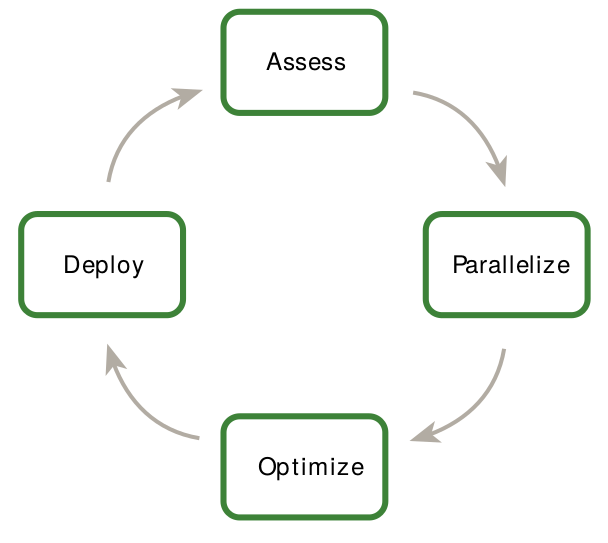
\includegraphics[width=5.0cm]{graphs/apod.png}
\end{center}
\end{frame}
%\input{algorithms.tex}
%\input{nsight.tex}
%\input{nvvp.tex}
%\input{nvcc.tex}
%\input{environment.tex}
%\input{thrust.tex}
%\input{openacc.tex}
%\input{libraries.tex}
%\input{library_advisor.tex}
\section{Conclusion}
\begin{frame}[fragile]
  \frametitle{Conclusion}
\begin{itemize}
  \item In this tutorials we covered most of the CUDA constructions that you need
    to start accelerating your program.
  \item However, before diving into such a low level programming and reinventing a wheel, 
    consider using existing accelerated libraries:
    \begin{itemize}
    \item \mycode{CUDA math library} that implements all the standard math functions
    \item \mycode{cuBLAS} - Basic Linear Algebra Subprograms
    \item \mycode{NVBLAS} - multigpu version of BLAS
    \item \mycode{cuFFT} - Fast Fourier Transform
    \item \mycode{nvGRAPH} - graph processing routines
    \item \mycode{cuRAND} - random numbers generators
    \item \mycode{cuSPARSE} - linear algebra for sparse matrices
    \item \mycode{NPP} - image, video processing
    \item \mycode{cuSOLVER} - higher level linear algebra routines on top of cuBlas and cuSparse
    \item \mycode{Magma} - Matrix Algebra on GPU and Multicore Architectures
    \item \mycode{AmgX} - Multi-Grid Accelerated Linear Solvers for Industrial Applications
    \item \mycode{ArrayFire} - signal and image processing
    \end{itemize}
\end{itemize}
\end{frame}

\begin{frame}[fragile]
  \frametitle{Conclusion}
\begin{itemize}
\item Continued:
\begin{itemize}
    \item \mycode{GUNROCK} - graph processing
    \item \mycode{GPP} - computational geometry 
    \item \mycode{CUB} - provides a collection of building blocks, includes sort, scan, reduction
    \item \mycode{cuDNN} - library for Deep Neural Networks
\end{itemize}
\item There are also higher level frameworks that make it easier to do GPU programming:
  \begin{itemize}
  \item \mycode{OpenACC} - high level pragma based framework for GPU acceleration, similar to OpenMP
  \item \mycode{Thrust} - C++ framework similar to STL
  \item \mycode{Kokkos} - another high-level C++ template library
  \end{itemize}
\end{itemize}
\end{frame}
\section{References}
\begin{frame}[fragile]
  \frametitle{References}
{\tiny
\begin{verbatim}
CUDA C Programming Guide:
https://docs.nvidia.com/cuda/pdf/CUDA_C_Programming_Guide.pdf

CUDA best practices:
https://docs.nvidia.com/cuda/pdf/CUDA_C_Best_Practices_Guide.pdf

Udacity "Introduction to Parallel Programming":
https://classroom.udacity.com/courses/cs344

Oxford course in CUDA programming:
https://people.maths.ox.ac.uk/gilesm/cuda/

Book: Programming massively parallel devices, 
by David B. Kirk, Wen-mei W. Hwu 

Thrust:
https://docs.nvidia.com/cuda/thrust/index.html

Book: Parallel Programming with OpenACC,
edited by Rob Farber
\end{verbatim}
}

\end{frame}


\section{Appendix: Tutorials on demand}
\begin{frame}[fragile]
  \frametitle{Appendix: Tutorials on demand}
  \begin{itemize}
    \item Currently the following tutorials are available at any time whenever there is an audience:
      \begin{enumerate}
        \item Introduction to Linux and RCC
        \item Introduction to Python
        \item Distributed MPI programming in C/C++/Python
        \item Multithreaded programming in OpenMP
        \item GPU programming with CUDA
        \item Introduction to Hadoop
        \item Big Data and Machine Learning with Spark and BigDL
        \item Deep Learning with Keras and TensorFlow
        \item Deep Learning with Theano
        \item Deep Learning with PyTorch
        \item Sequence Models with Recurrent Neural Networks
        \item Reinforcement Learning
        \item Singularity Container
      \end{enumerate}
    \item More are coming: Autoencoders, Generative Adversarial Networks, Object detection with YOLO, C++, ...
    \item Requests for other topics?
  \end{itemize}
\end{frame}


\end{document}
